\documentclass[a4paper,twocolumn]{IEEEtran}

\usepackage{amsmath,amsfonts,amssymb}
\usepackage{graphicx,float,subfig}
\usepackage{booktabs}
\usepackage[colorlinks=true]{hyperref}

\author{Oliver Kirkpatrick\footnote{oliver.kirkpatrick@rmit.edu.au}}

\begin{document}
    \title{Analysis of Gamma Ray Spectra from Reference Isotopes with Multi-Channel Analyzers}
    \author{\IEEEauthorblockA{Oliver Kirkpatrick}
    \\
    \IEEEauthorblockA{School of Engineering, RMIT University\\
    Email: s3725341@student.rmit.edu.au}}

    \maketitle
    \begin{abstract}
        The interaction of gamma rays with matter, the results are classed into three categories: photoelectric scattering, Compton Scattering, and Pair production. Which of these effects occurs is closely linked with the energy carried by the original gamma ray. Presented in this study is an investigation into gamma ray scattering and spectra using a Thallium doped Sodium Iodide (NaI(Tl)) scintillating crystal detector, and a multi-channel analyzer. Common radioactive isotopes of Cesium, Sodium, and Cobalt were utilized as reference isotopes to calibrate the equipment setup, such that an unknown material could be identified through gamma ray spectra and half life.
    \end{abstract}
    \section{Introduction}
    \begin{itemize}
    \item Gamma ray scattering is a phenomenon that occurs when gamma rays interact with matter.
    \item The process involves the deflection of gamma rays from their original path due to interactions with atomic nuclei.
    \item The scattering of gamma rays is caused by the electromagnetic interaction between the gamma rays and atomic electrons.
    \item The probability of scattering depends on the energy of the gamma rays and the atomic number of the material being scattered.
    \item Scattering can occur at any angle and is described by a scattering cross-section.
    \item The scattering cross-section is a measure of the probability of scattering and is dependent on the energy of the gamma ray.
    \item Gamma ray scattering is used in many applications, including medical imaging and materials science.
    \item In medical imaging, gamma ray scattering is used to identify the presence and location of tumors or other abnormalities.
    \item Materials science researchers use gamma ray scattering to study the atomic structure of materials.
    \item Gamma ray scattering is also used in astrophysics to study the properties of celestial objects.
    \item For incident gamma rays with lower energies ($<100$ keV), this photoelectric effect is dominant~\cite{kane1986elastic,kane2005elastic}
    \item The Compton effect is a type of gamma ray scattering in which a gamma ray loses energy and changes direction after interacting with an atomic electron.
    \item The energy lost by the gamma ray in the Compton effect is transferred to the electron, which is ejected from the atom.
    \item The Compton effect is the dominant mechanism for gamma ray scattering at intermediate energies.
    \item At high energies, gamma rays can also undergo pair production, in which a gamma ray is converted into an electron-positron pair.
    \item Gamma ray scattering is an important phenomenon in physics and has many practical applications in science and medicine.
    \end{itemize}
        
    \section{Results and Discussion}
    \subsection{Calibration Process}
    \begin{figure}[H]
        \centering
        \subfloat[$^{137}$Cs Gamma Ray Spectra\label{subfig:cs-137-grs}]{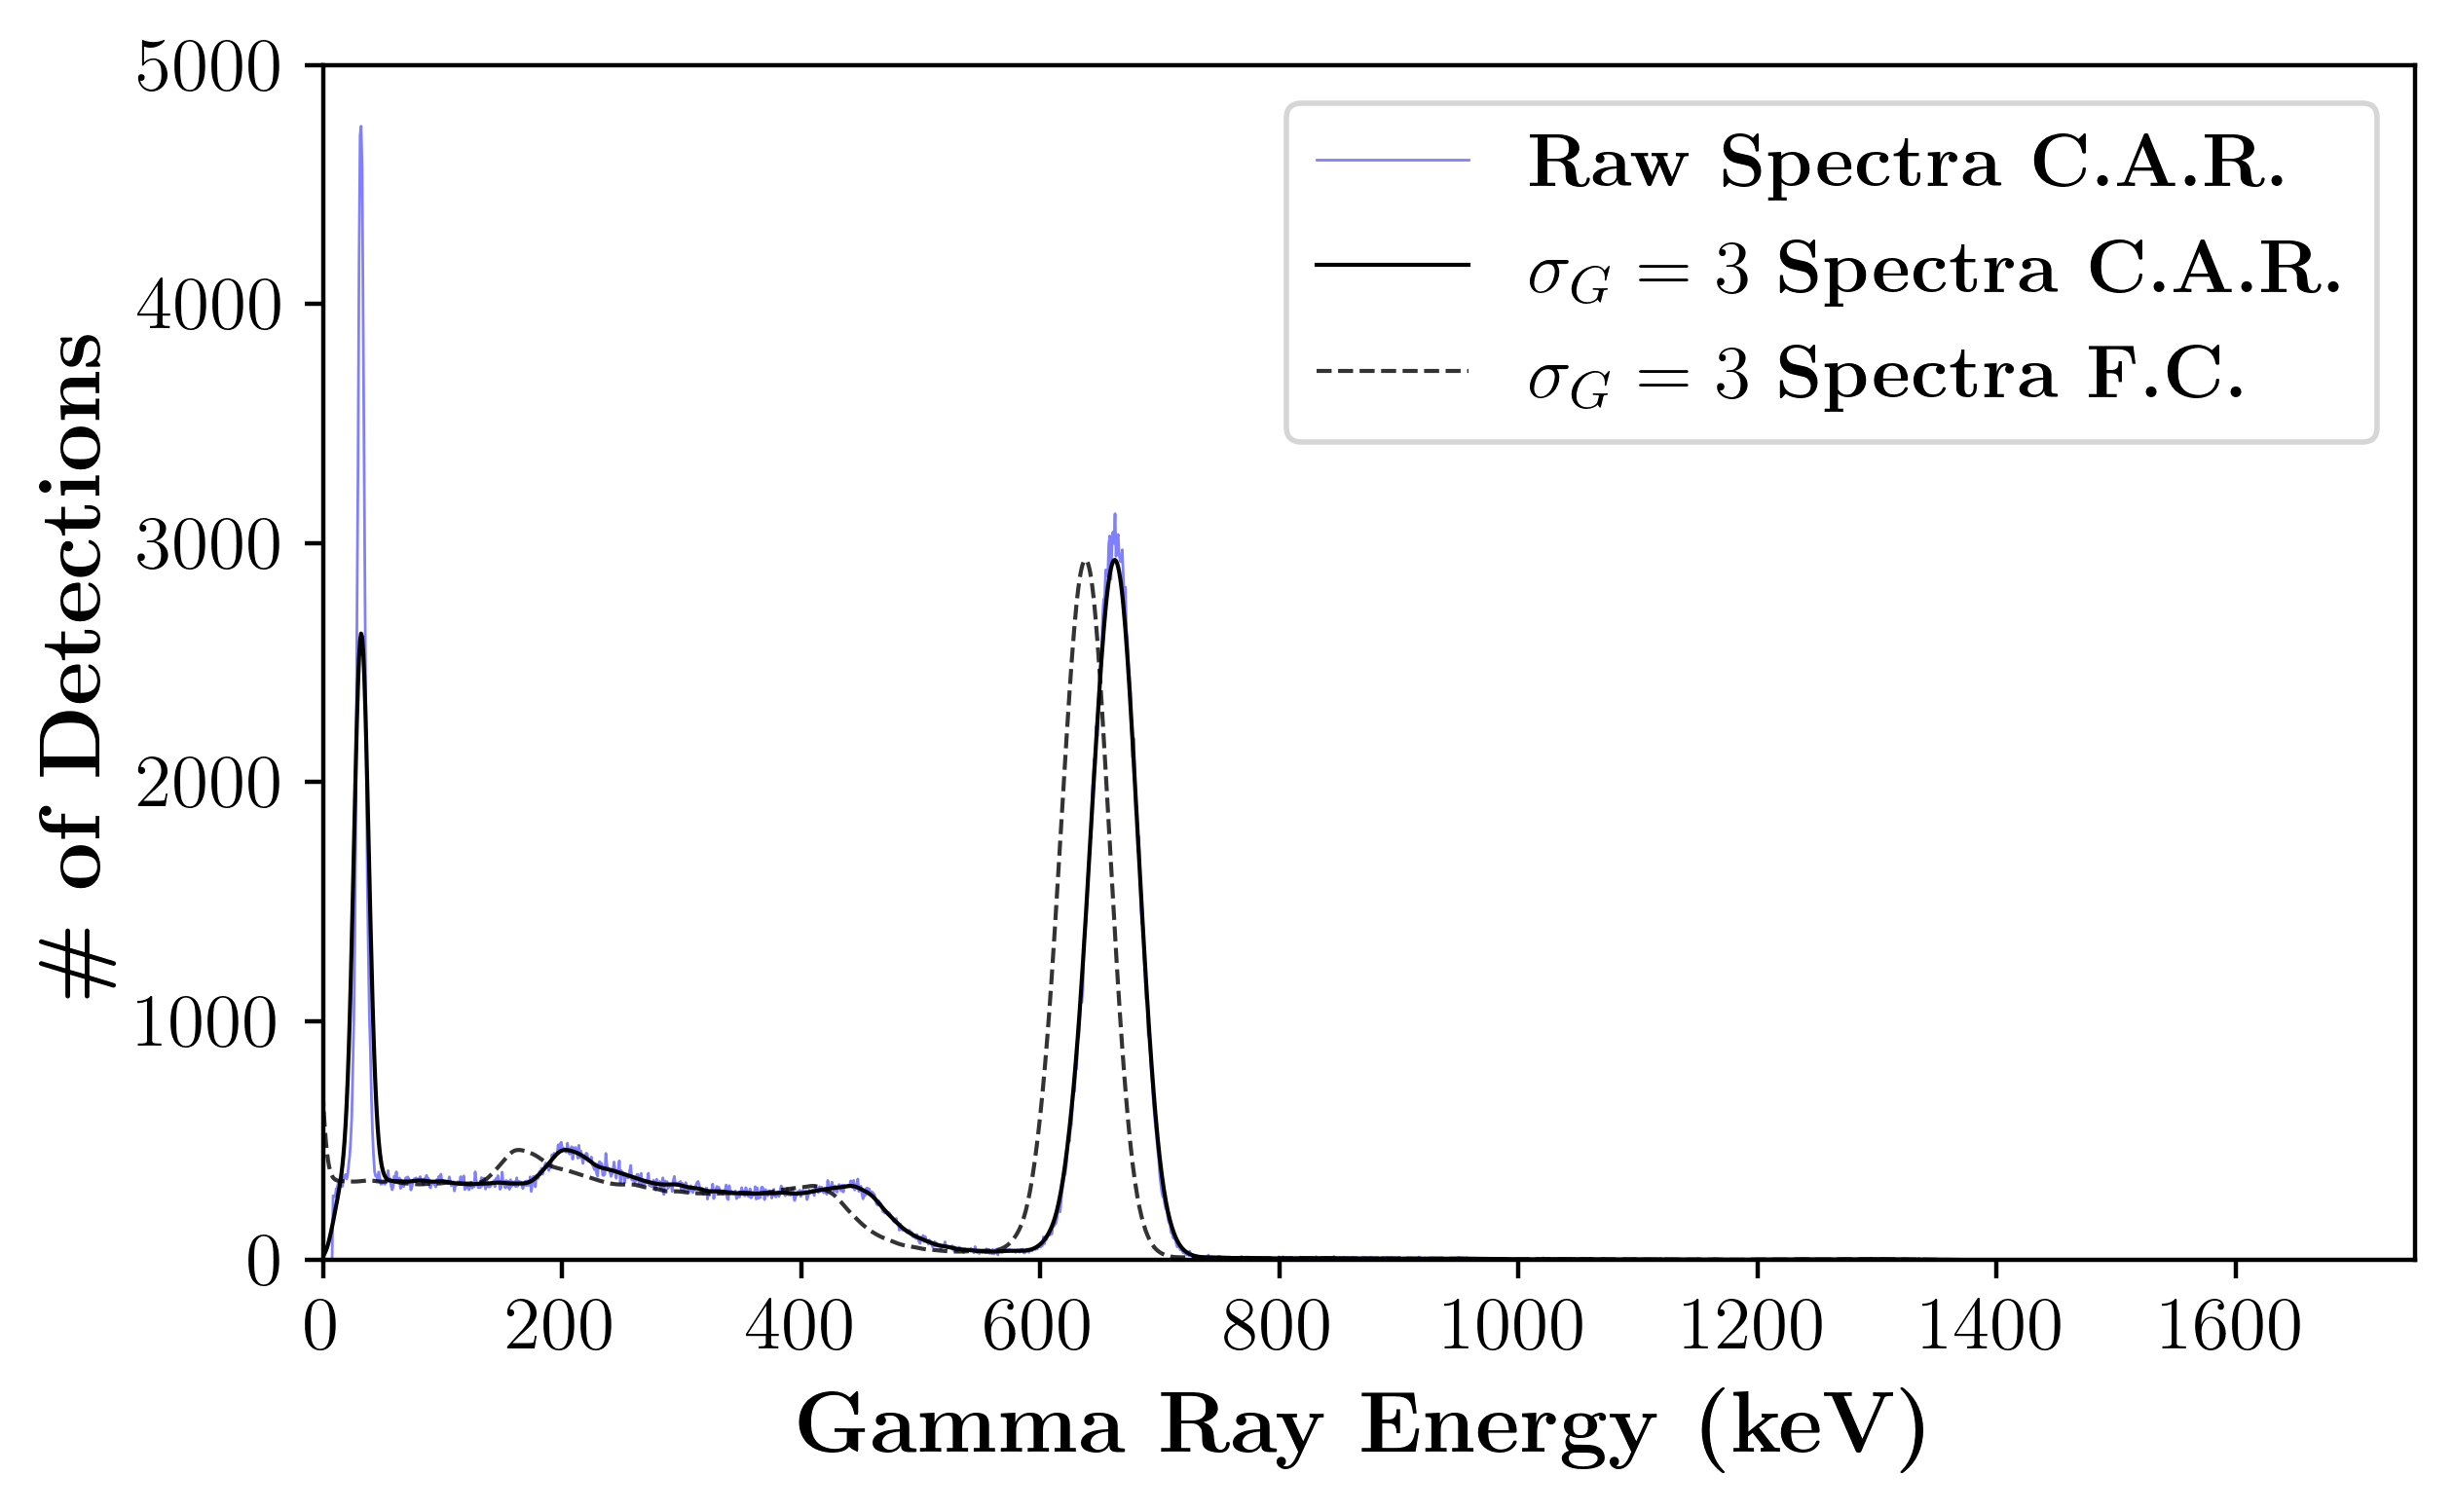
\includegraphics[width=0.95\linewidth]{figures/calibration_spectrum_cs_counts_overlay_both_mca.png}}\\
        \subfloat[$^{22}$Na Gamma Ray Spectra\label{subfig:na-22-grs}]{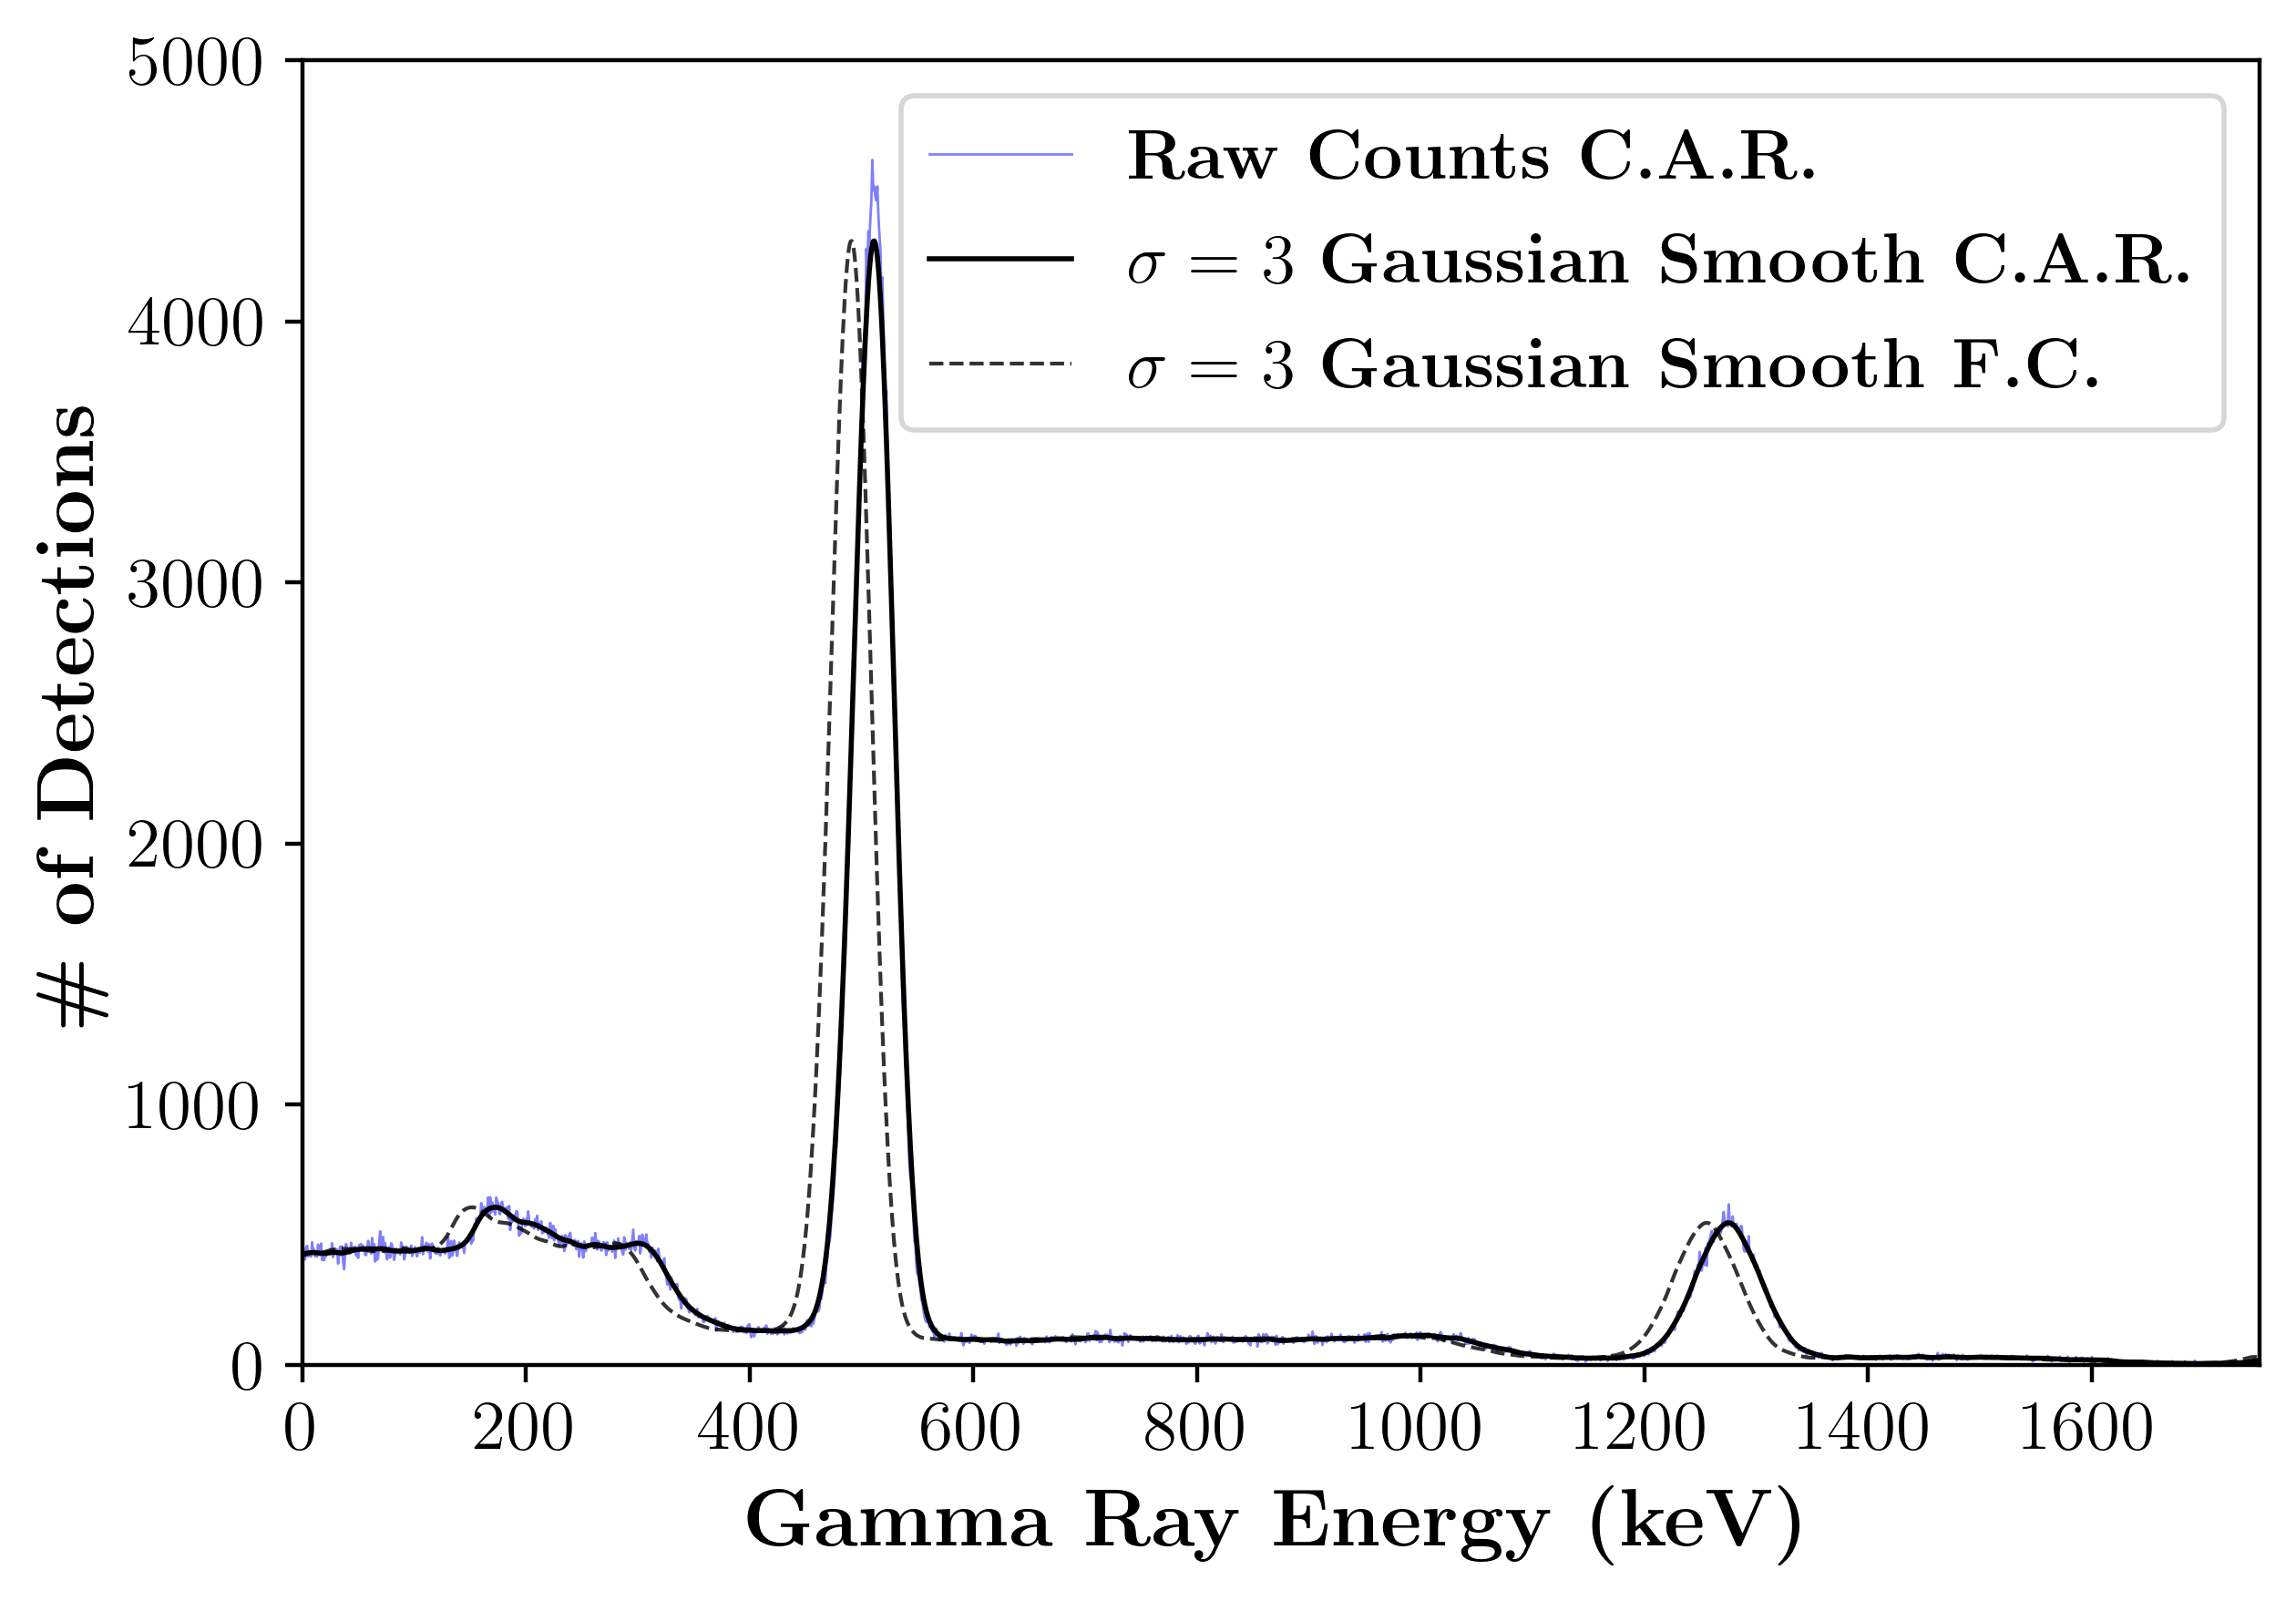
\includegraphics[width=0.95\linewidth]{figures/calibration_spectrum_na_counts_overlay_both_mca.png}}\\
        \subfloat[$^{60}$Co Gamma Ray Spectra\label{subfig:co-60-grs}]{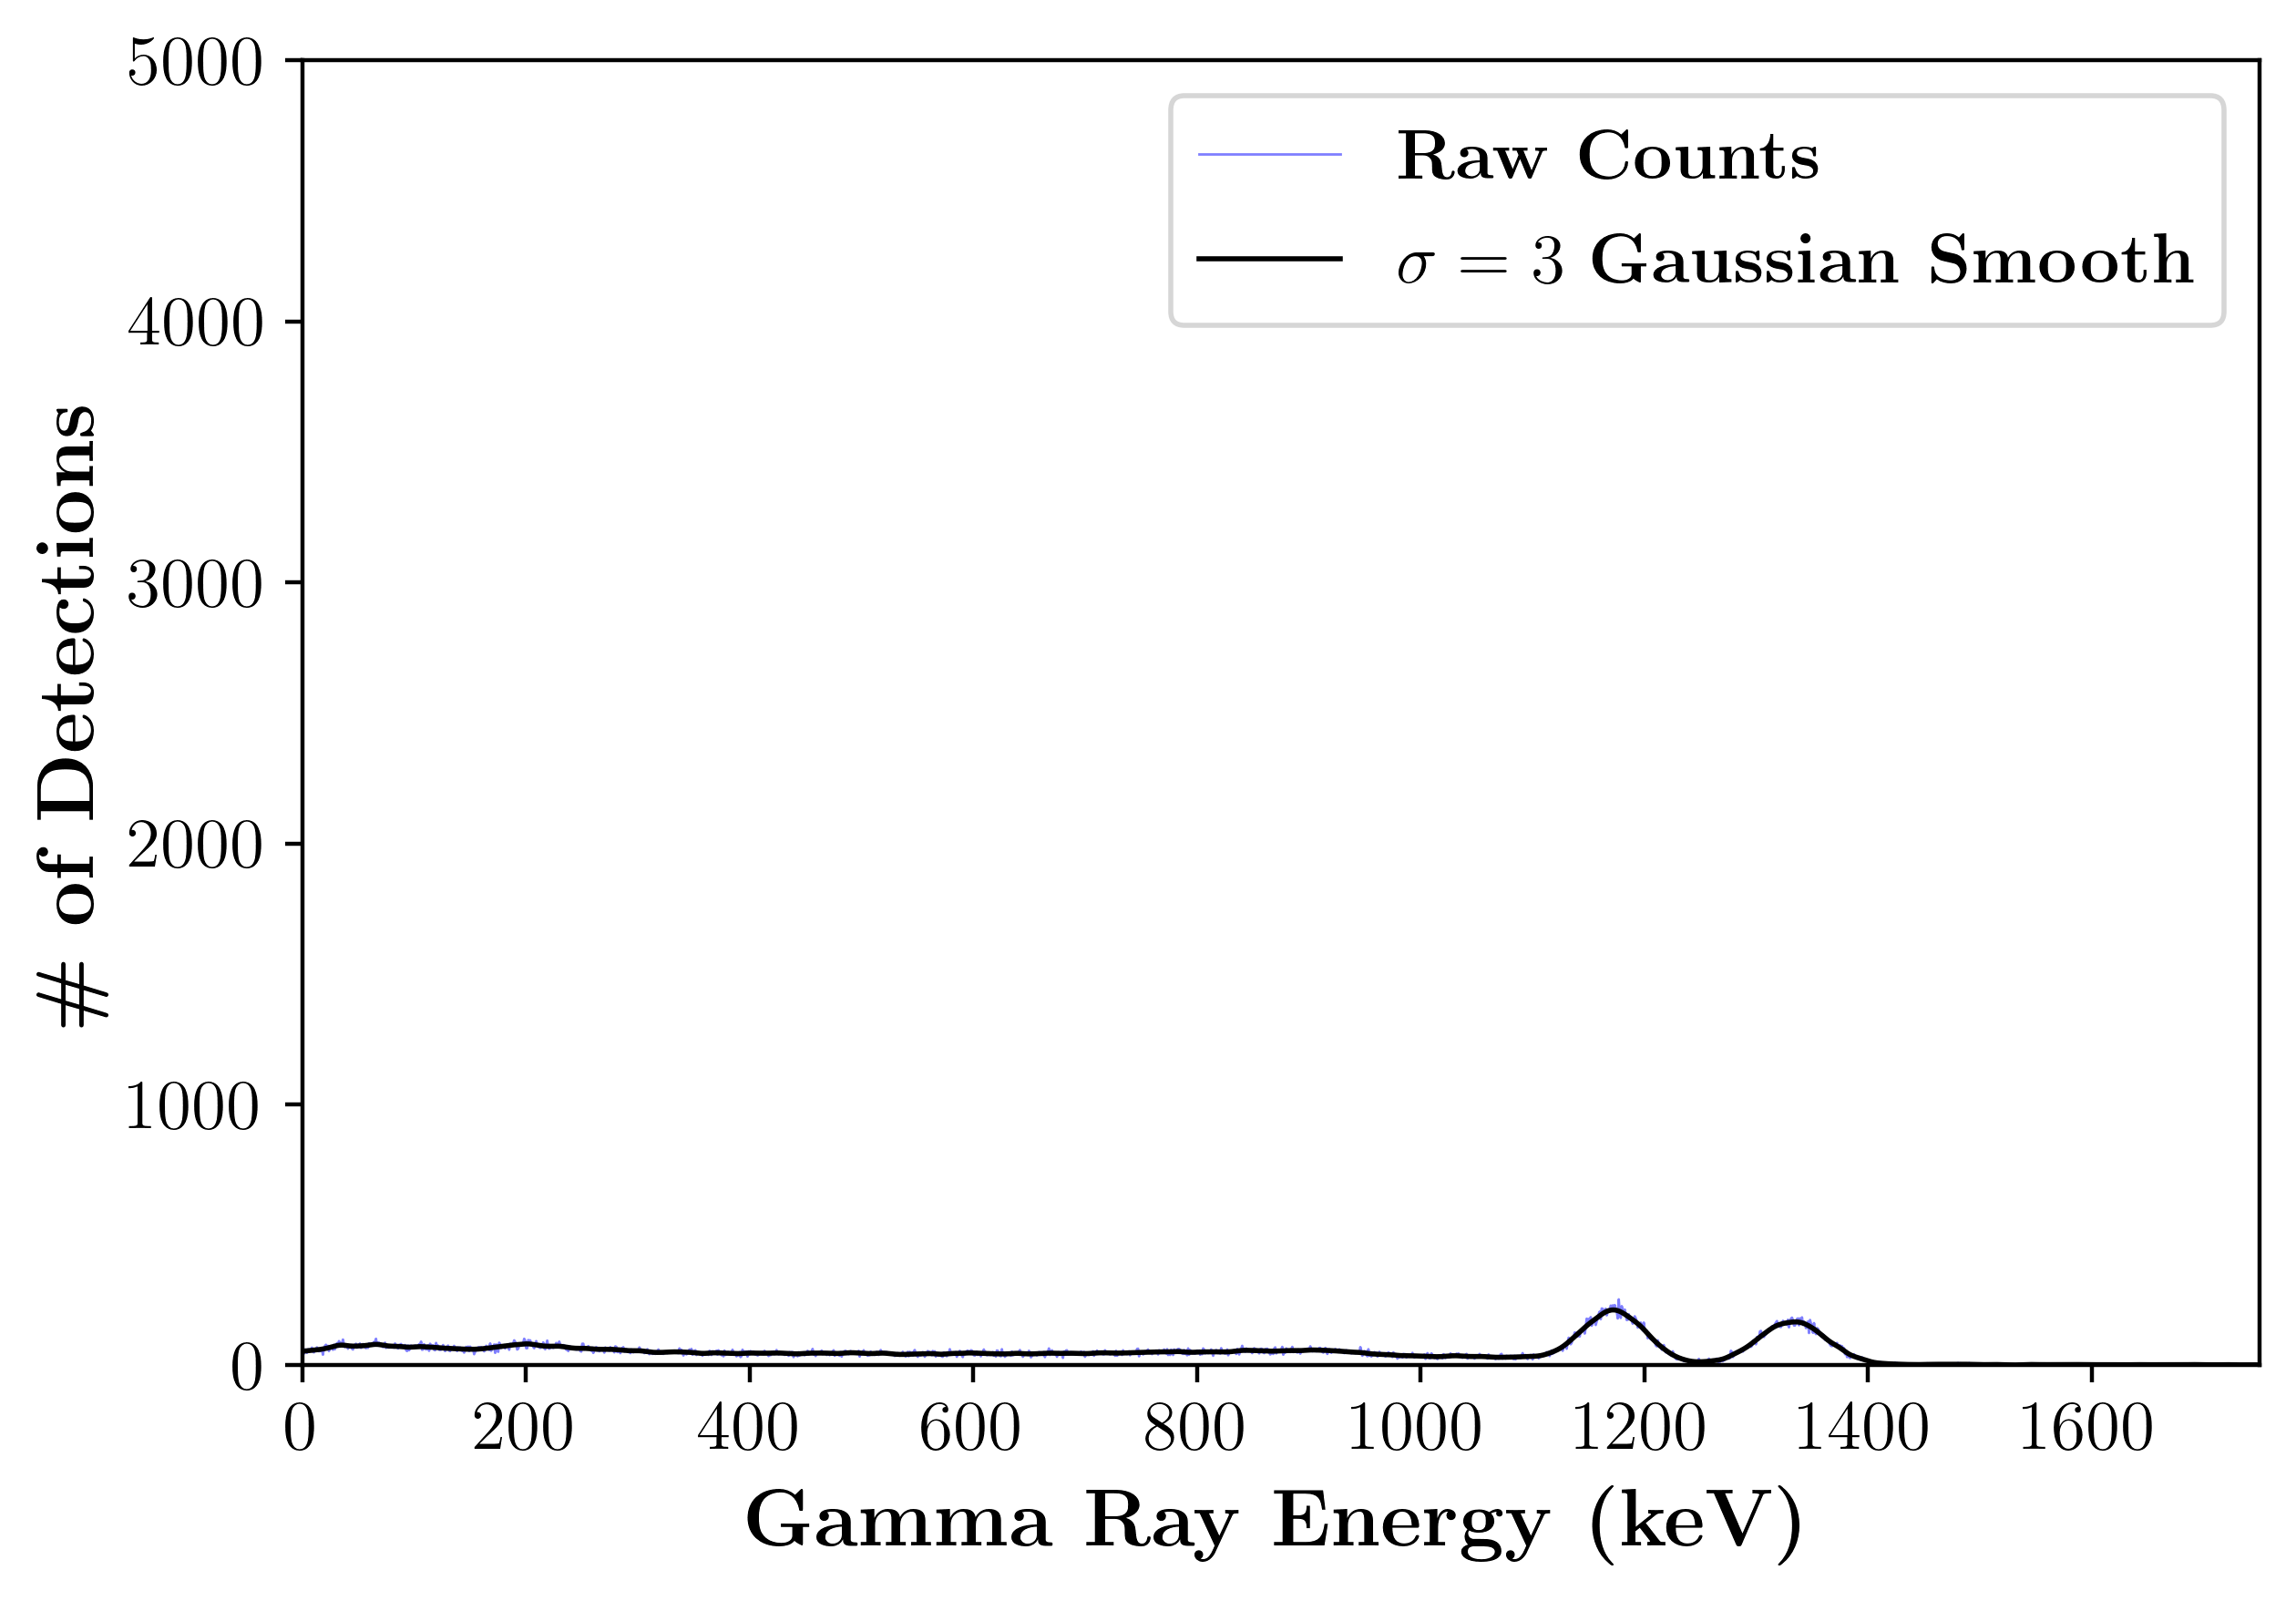
\includegraphics[width=0.95\linewidth]{figures/calibration_spectrum_co_counts_overlay_final_mca.png}}
        \caption{Gamma ray spectra for known isotopes of Cesium ($^{137}$Cs), Sodium ($^{22}$Na), and Cobalt ($^{60}$Co). Cobalt was the final isotope tested, and the calibration metrics calculated for it were used for the rest of the experiment. For the Cesium and Sodium isotopes, the spectra with the calibration at recording (\textbf{C.A.R.}), is shown in solid black, and the spectra adjusted with the final calibration (\textbf{F.C.}) is shown in dashed gray. Raw counts for all isotopes are shown in blue, though these are often obscurred by the $\sigma=3$ gaussian smoothed curves.}
    \end{figure}
    \subsection{Background Radiation}
    \begin{figure}[H]
        \centering
        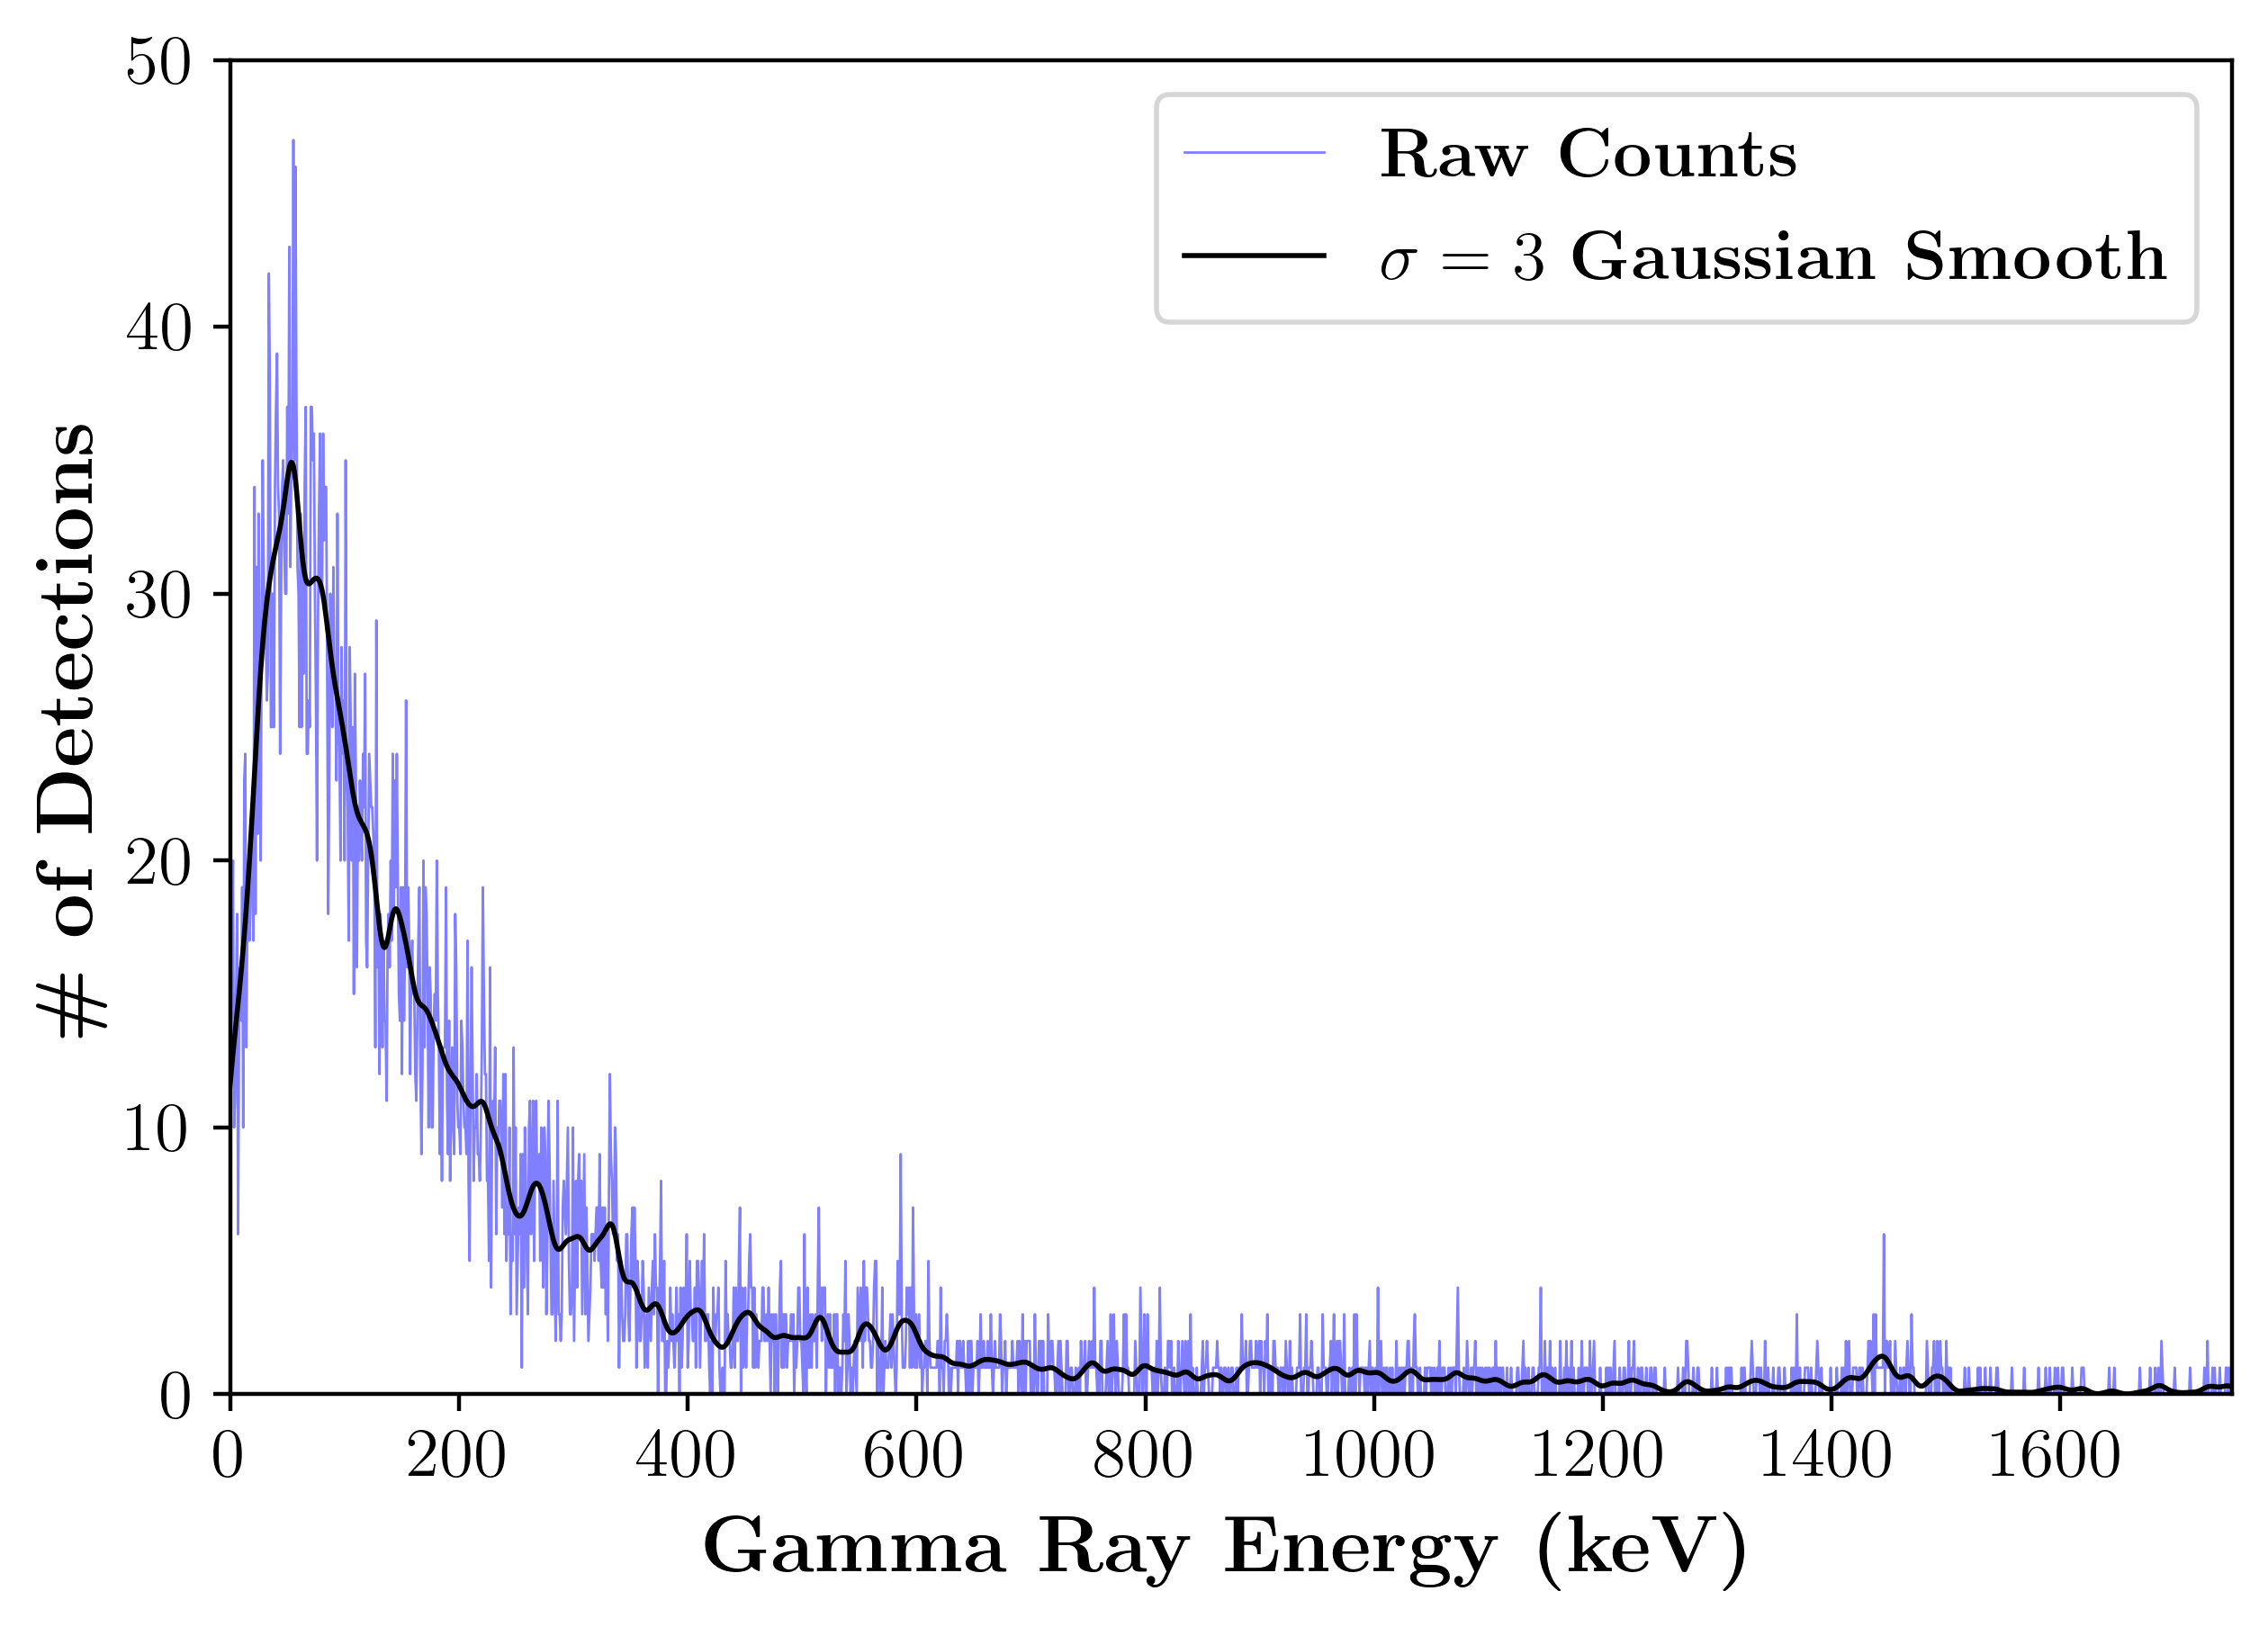
\includegraphics[width=0.95\linewidth]{figures/background_counts_overlay.png}
        \caption{Background radiation profile.}
    \end{figure}
    \subsection{Analysis of Unknown Sample}
    \begin{figure}[H]
        \centering
        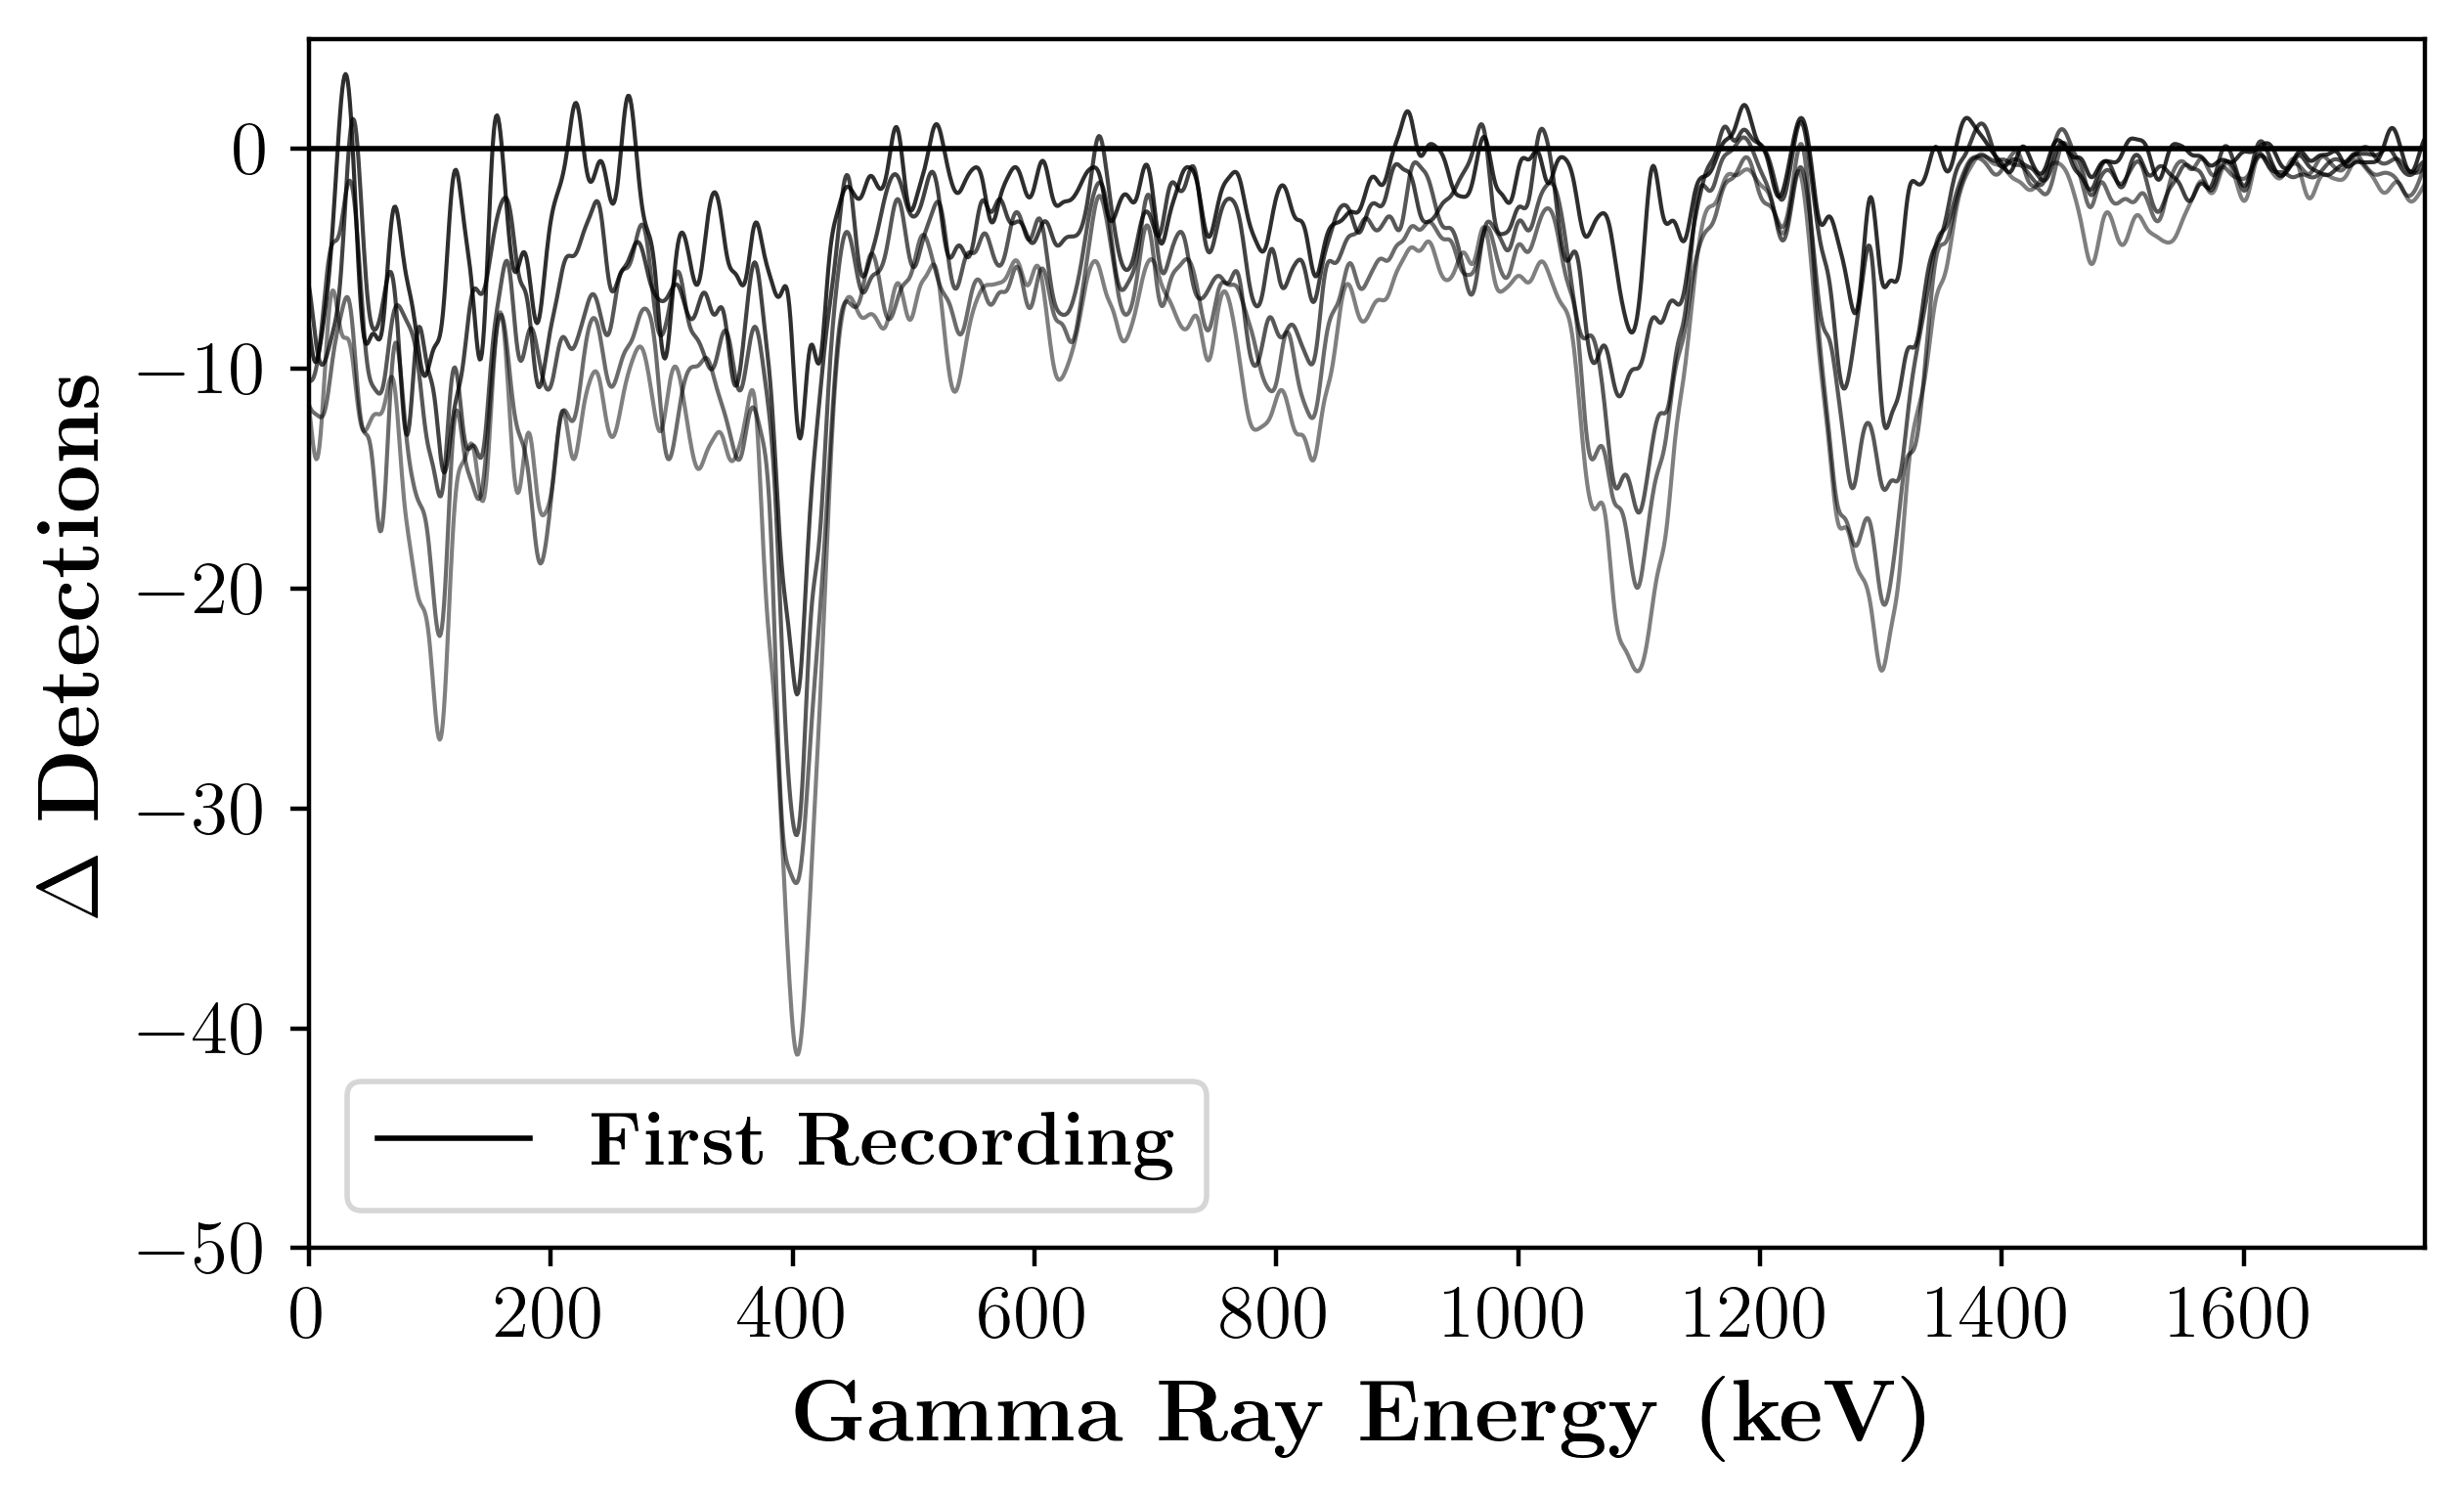
\includegraphics[width=0.95\linewidth]{figures/difference_counts_smooth.png}
    \end{figure}

    \begin{table*}[t]
        \centering
        \caption{Total counts and peak energies with with increasing time since first measurement.}
        \begin{tabular}{c c c c c c c}
            \toprule
            \textbf{Sample Number} & $T+$ \textbf{(s)} & \textbf{Total Counts} & \textbf{Peak 1 Energy} & \textbf{Peak 2 Energy} & \textbf{Peak 3 Energy} & \textbf{Peak 4 Energy} \\
            \midrule
            1 & 0s & 68493 & 401.24 keV &  815.92 keV & 1096.59 keV & 1296.46 keV \\
            2 & 420s & 63755 & 400.52 keV & 799.32 keV & 1106.59 keV & 1295.25 keV \\
            3 & 819s & 59850 & 401.25 keV & 796.80 keV & 1099.32 keV  & 1293.16 keV \\
            4 & 1199s & 56863 & 400.35 keV & 759.04 keV & 1097.07 keV & 1295.73 keV \\
            5 & 1559s & 53111 & 401.94 keV & 805.54 keV & 1104.55 keV & 1296.78 keV \\
            6 & 1936s & 50483 & 400.41 keV & 812.17 keV & 1085.92 keV & 1292.84 keV \\
            \bottomrule
        \end{tabular}
        \label{tab:counts_v_time}
    \end{table*}
    \bibliography{ref}
    \bibliographystyle{apalike}
    \onecolumn
    \appendix
    \begin{figure}[H]
        \centering
        \subfloat[Recording 1, hh:mm:ss, $T+$ minutes\label{subfig:mystery-recording-1}]{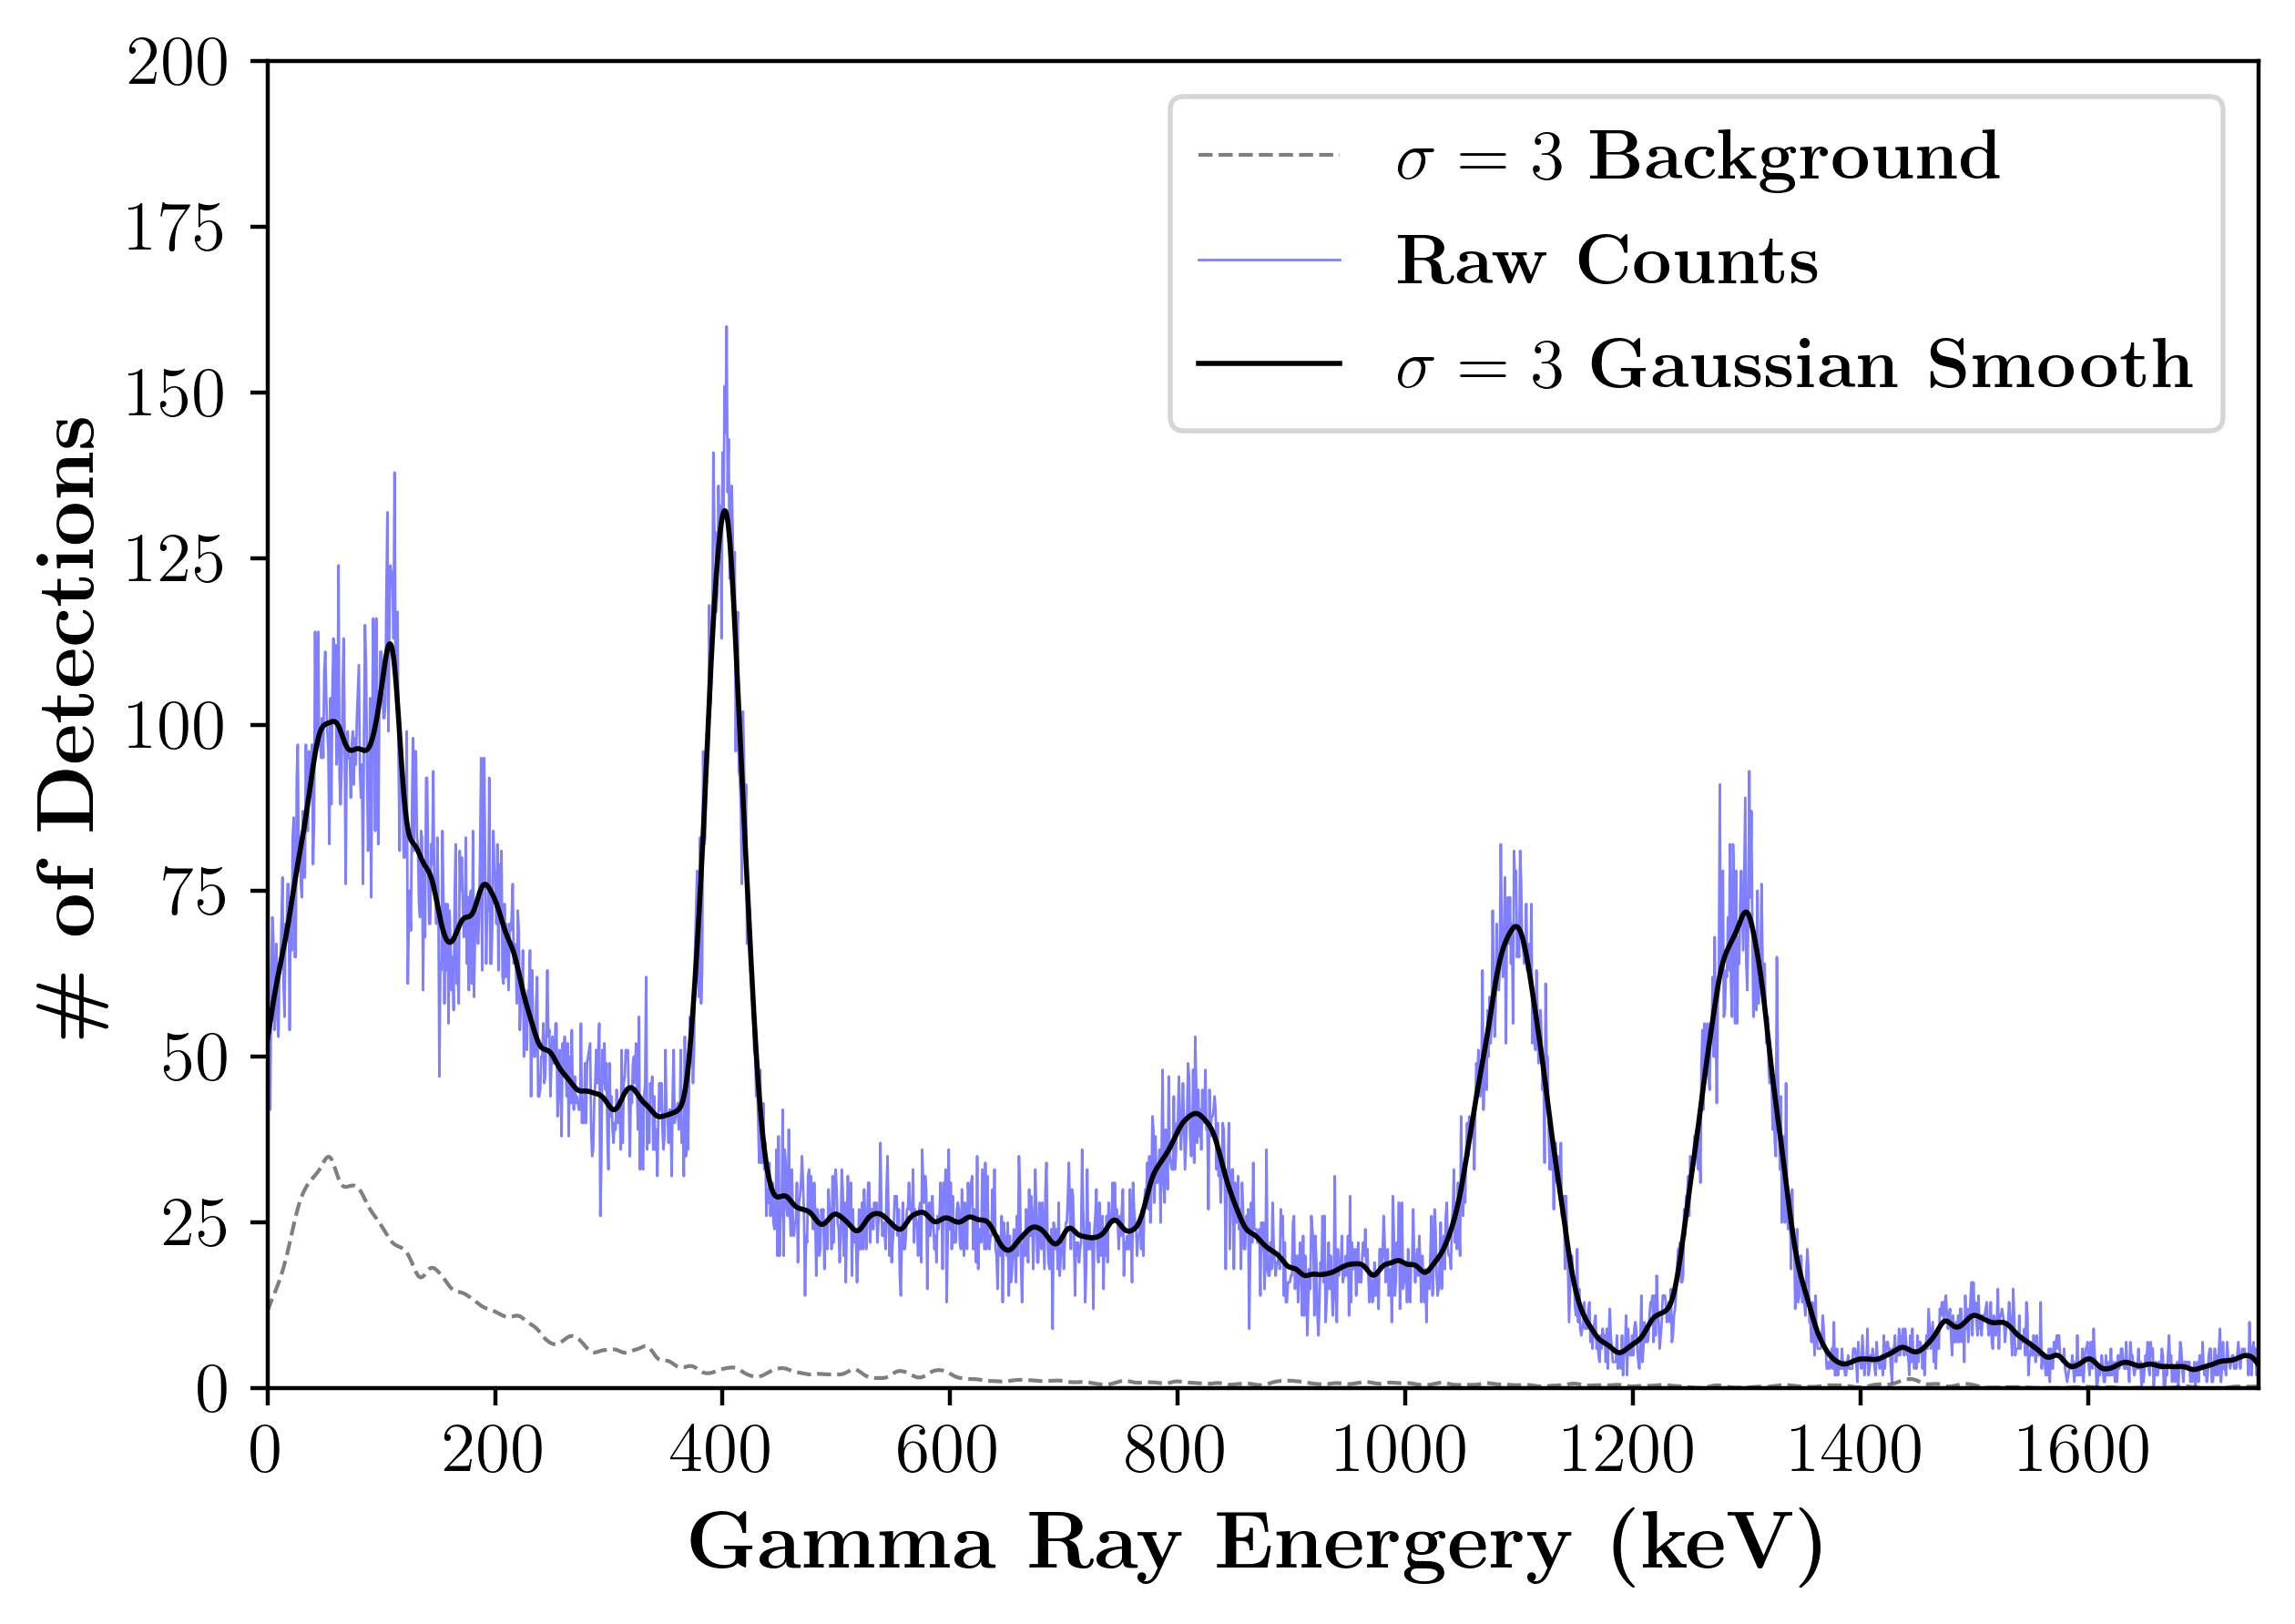
\includegraphics[width=0.49\textwidth]{figures/mystery_1_background_counts_overlay.png}}
        \hspace{\fill}
        \subfloat[Recording 2, hh:mm:ss, $T+$ minutes\label{subfig:mystery-recording-2}]{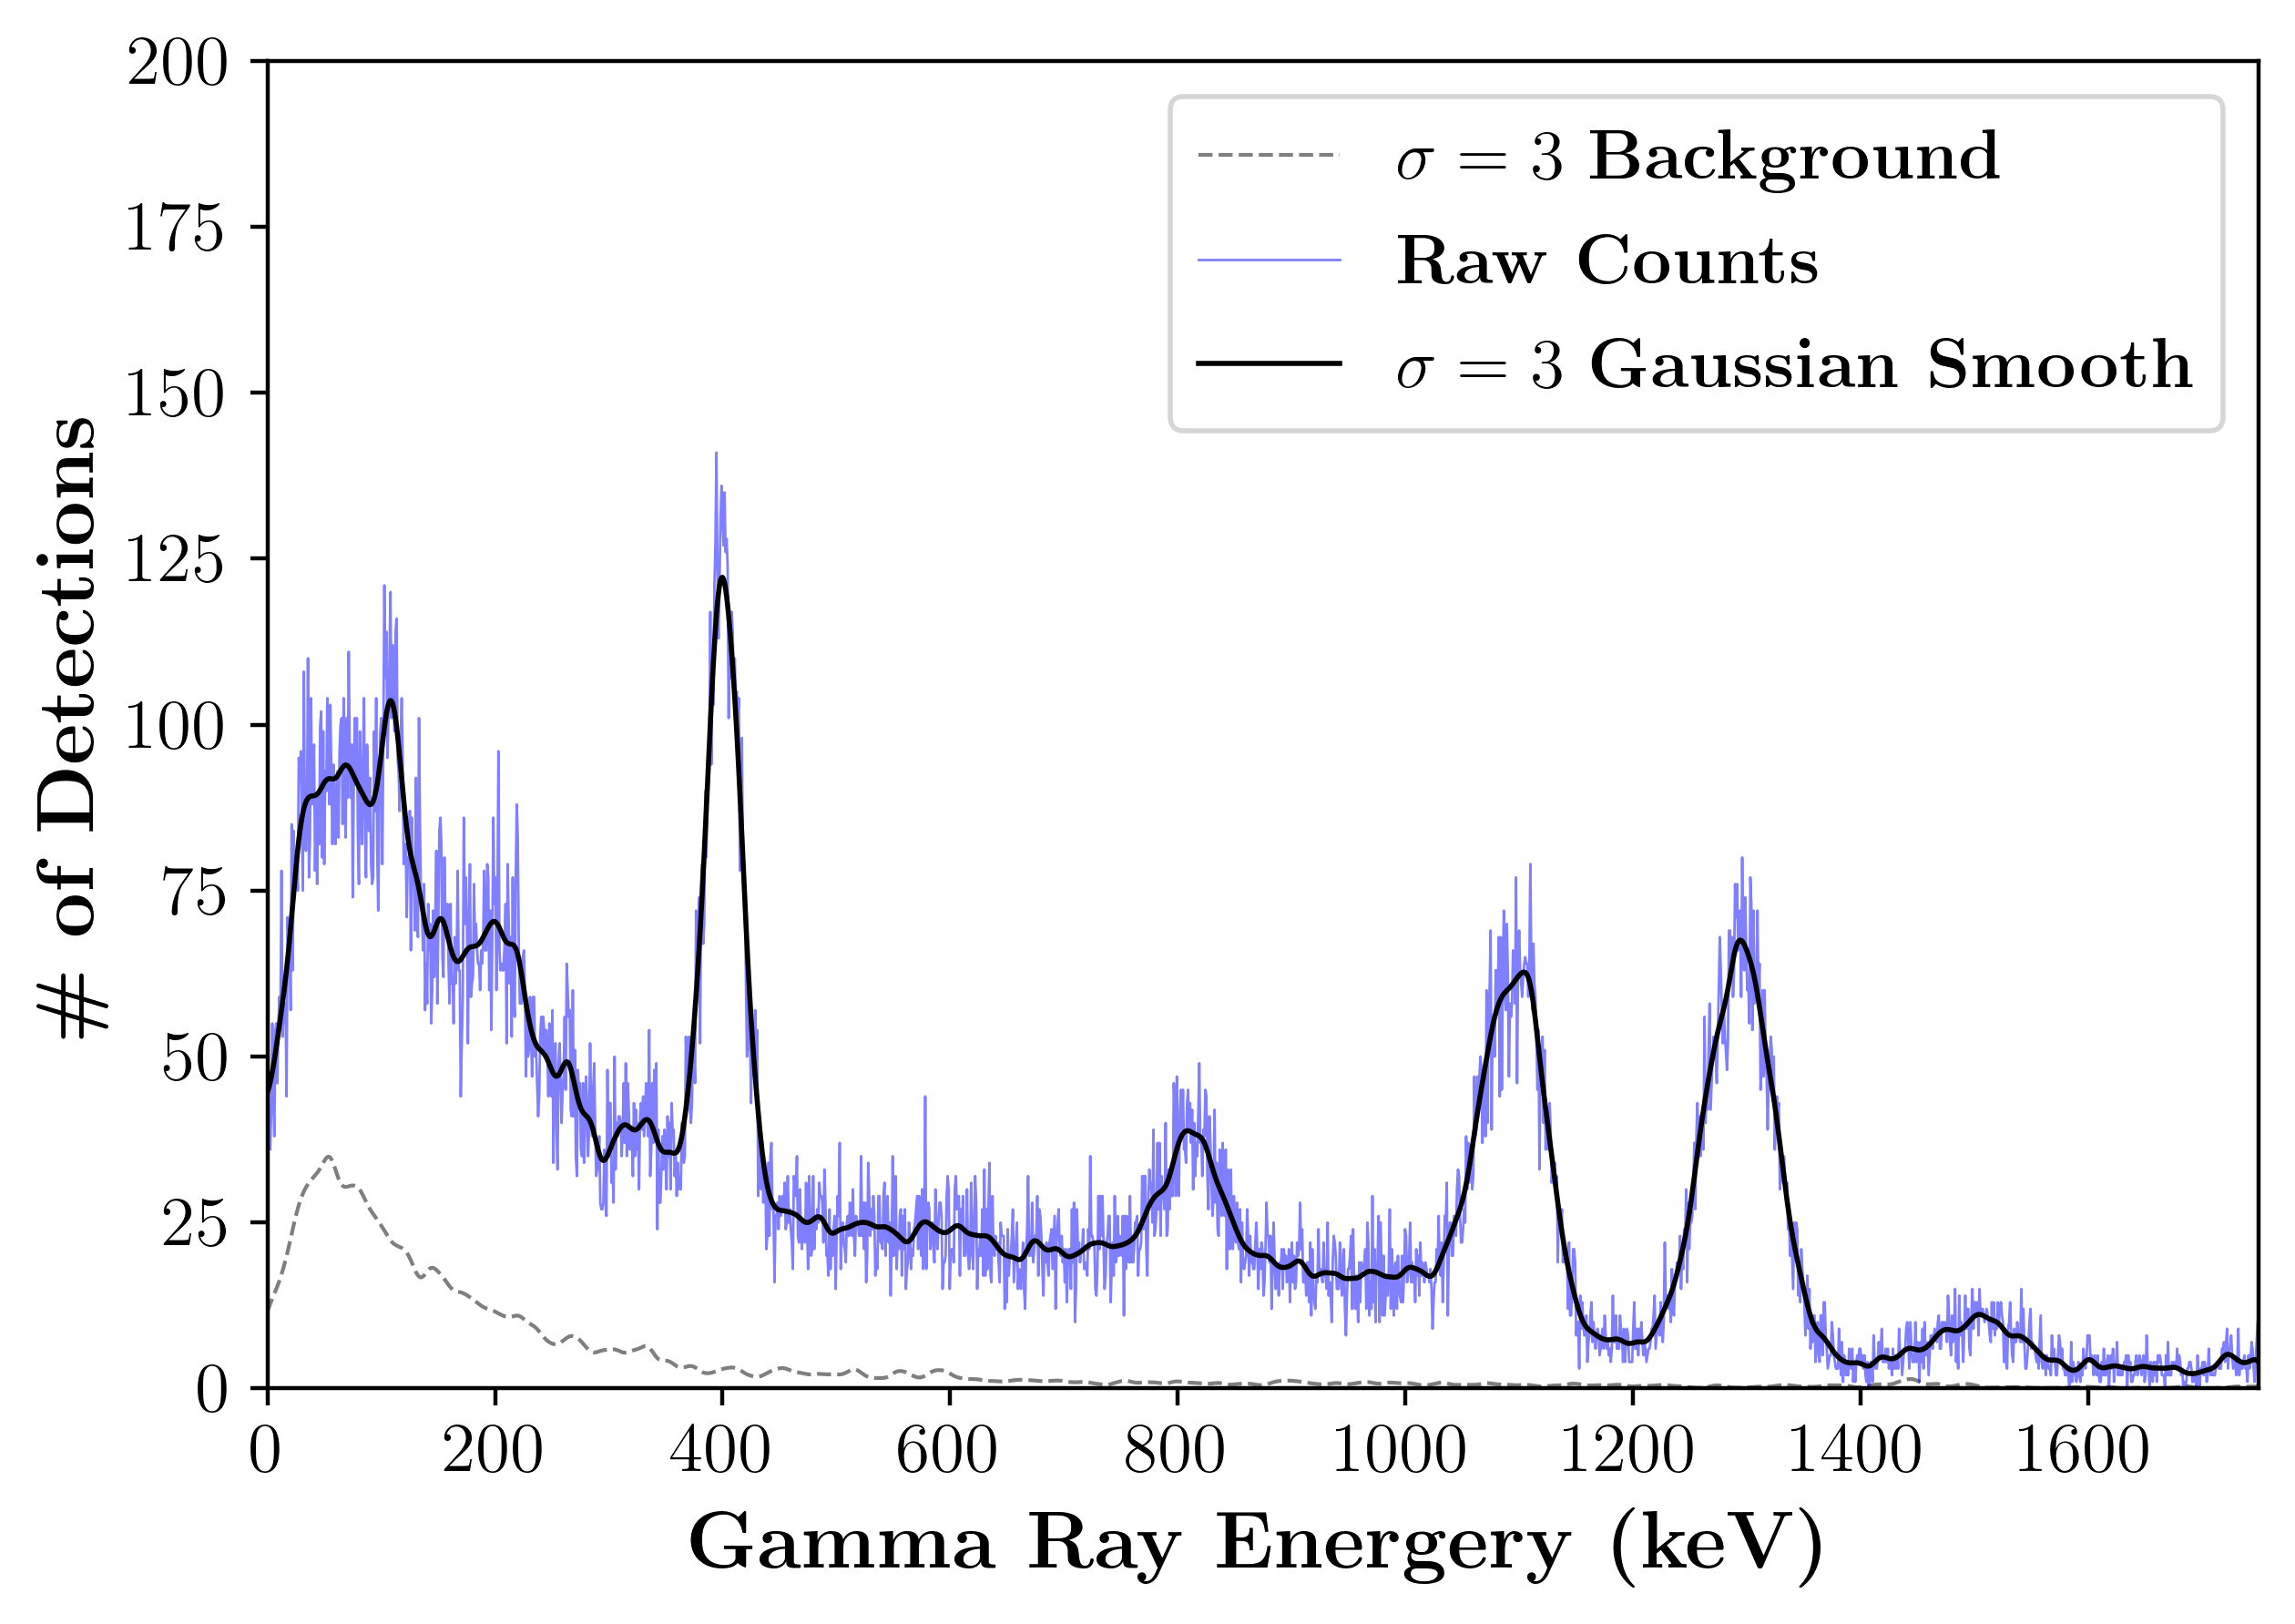
\includegraphics[width=0.49\textwidth]{figures/mystery_2_background_counts_overlay.png}}\\
        \subfloat[Recording 3, hh:mm:ss, $T+$ minutes\label{subfig:mystery-recording-3}]{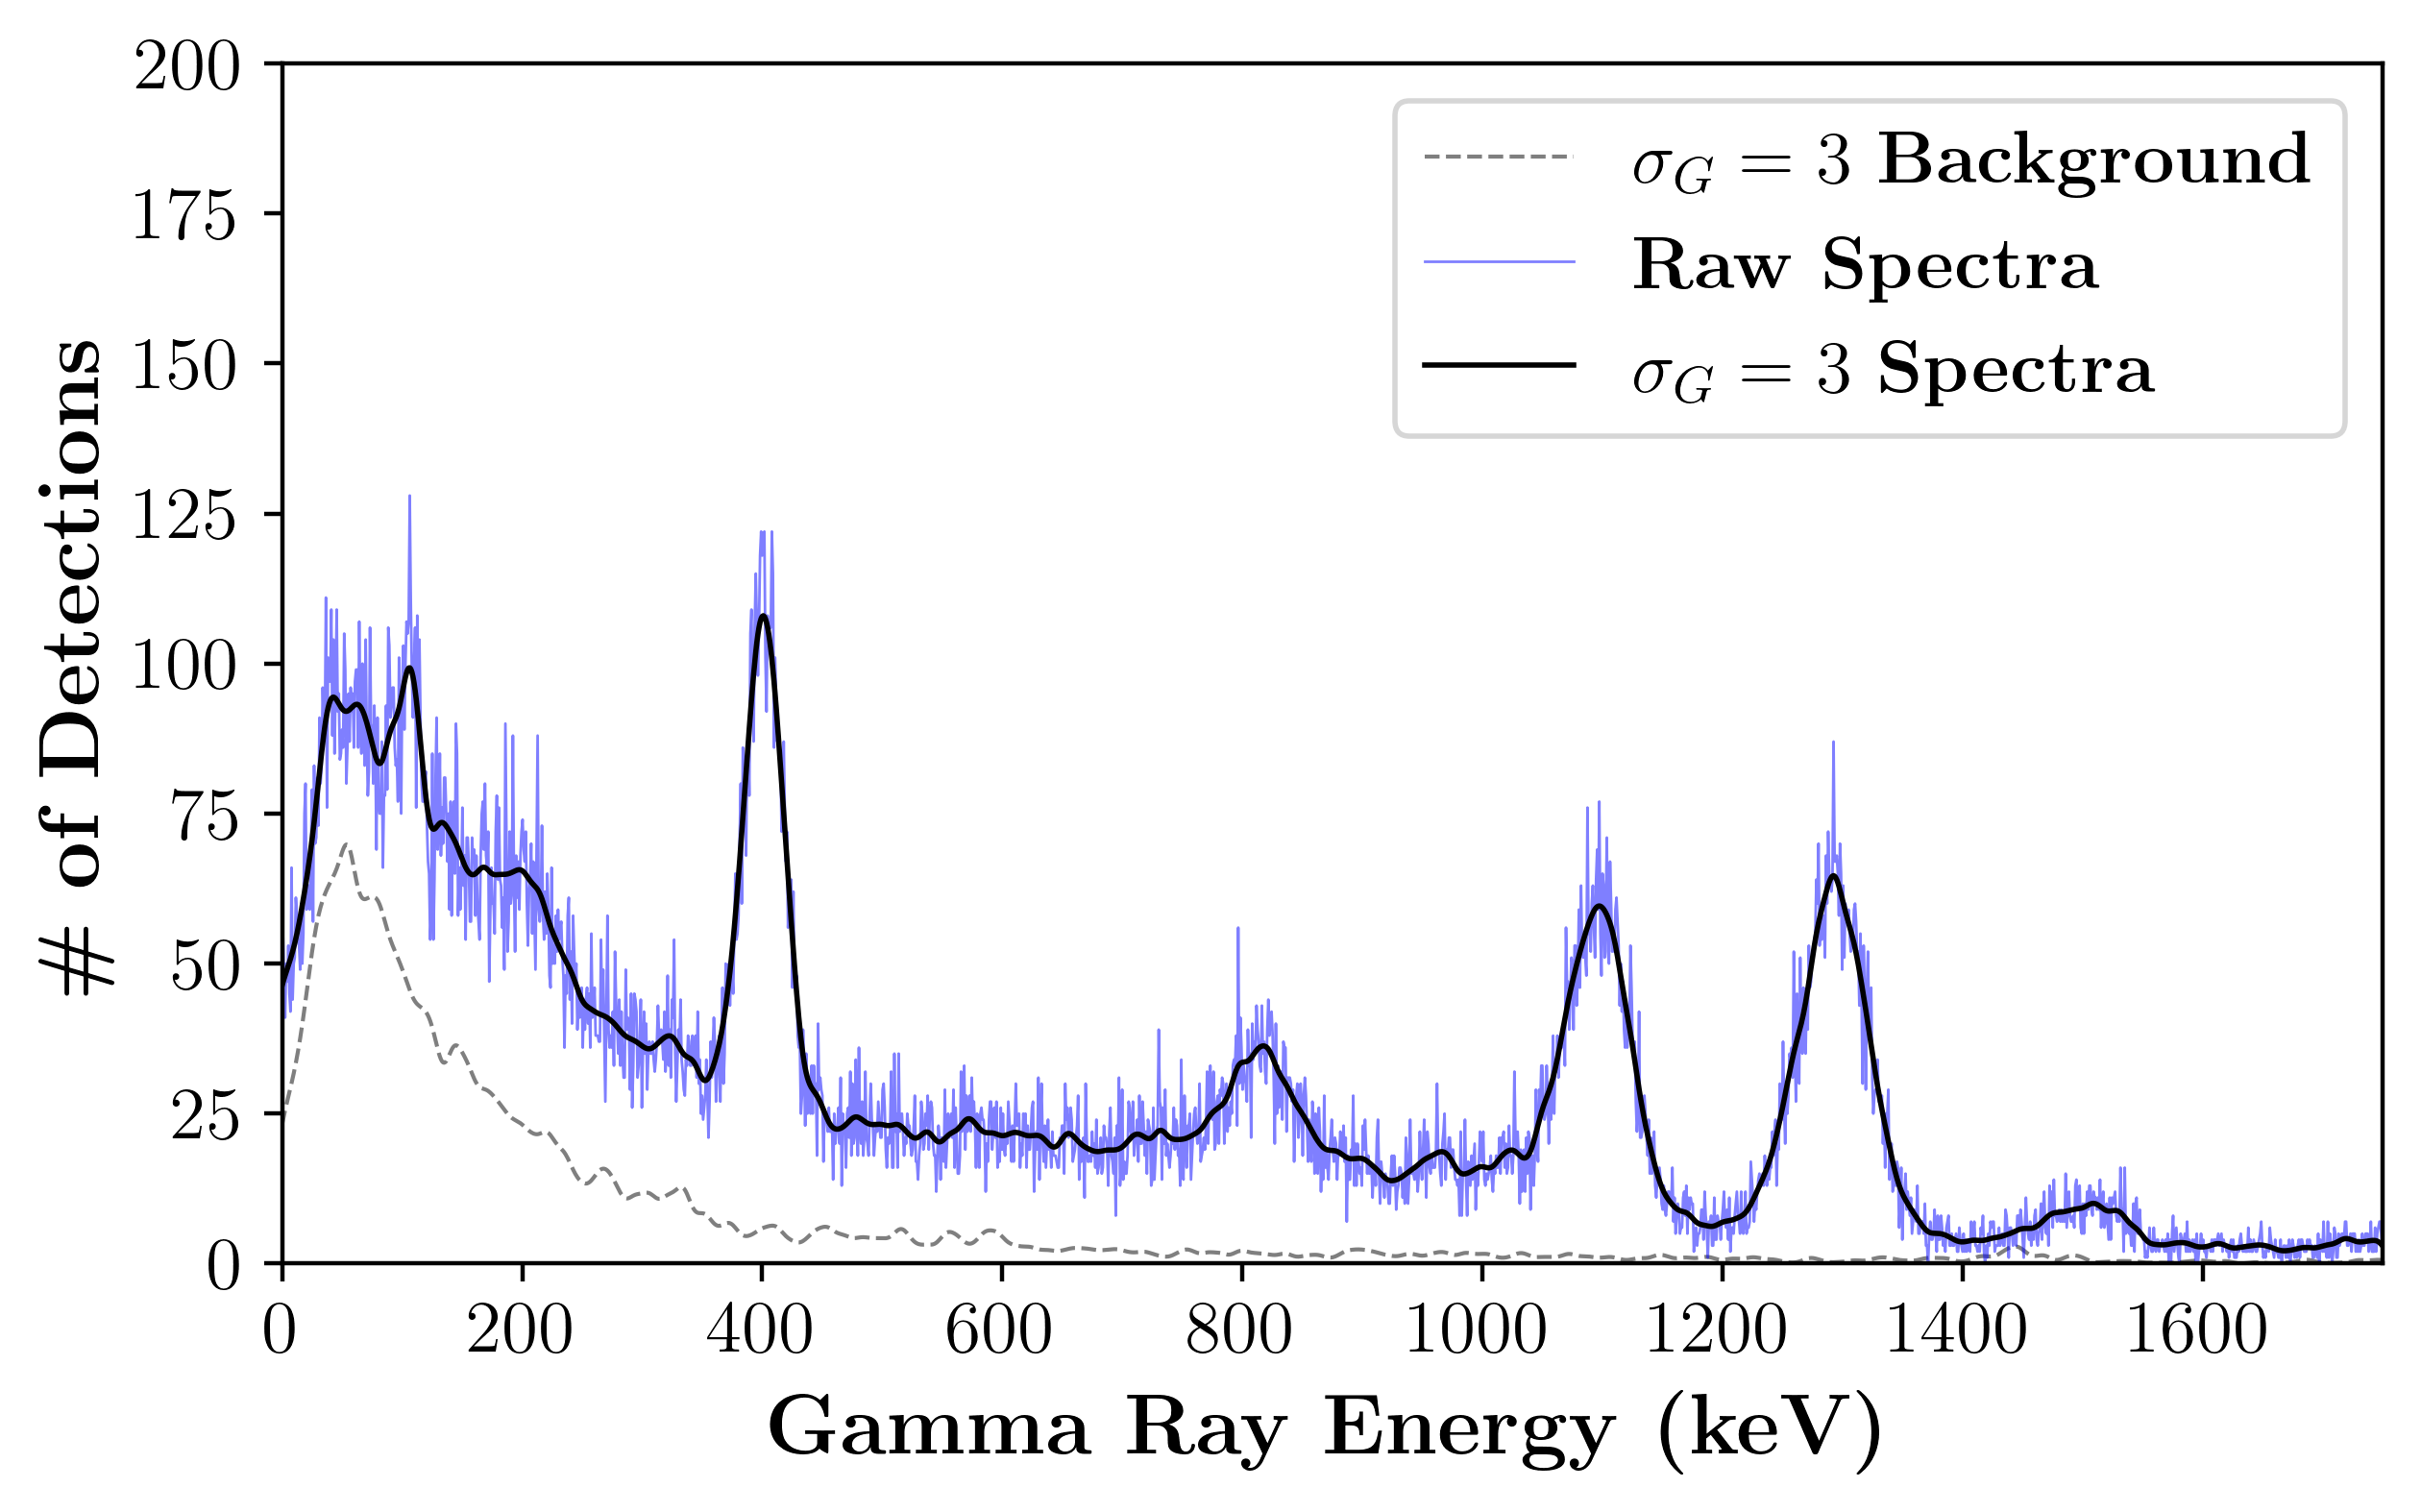
\includegraphics[width=0.49\textwidth]{figures/mystery_3_background_counts_overlay.png}}
        \hspace{\fill}
        \subfloat[Recording 4, hh:mm:ss, $T+$ minutes\label{subfig:mystery-recording-4}]{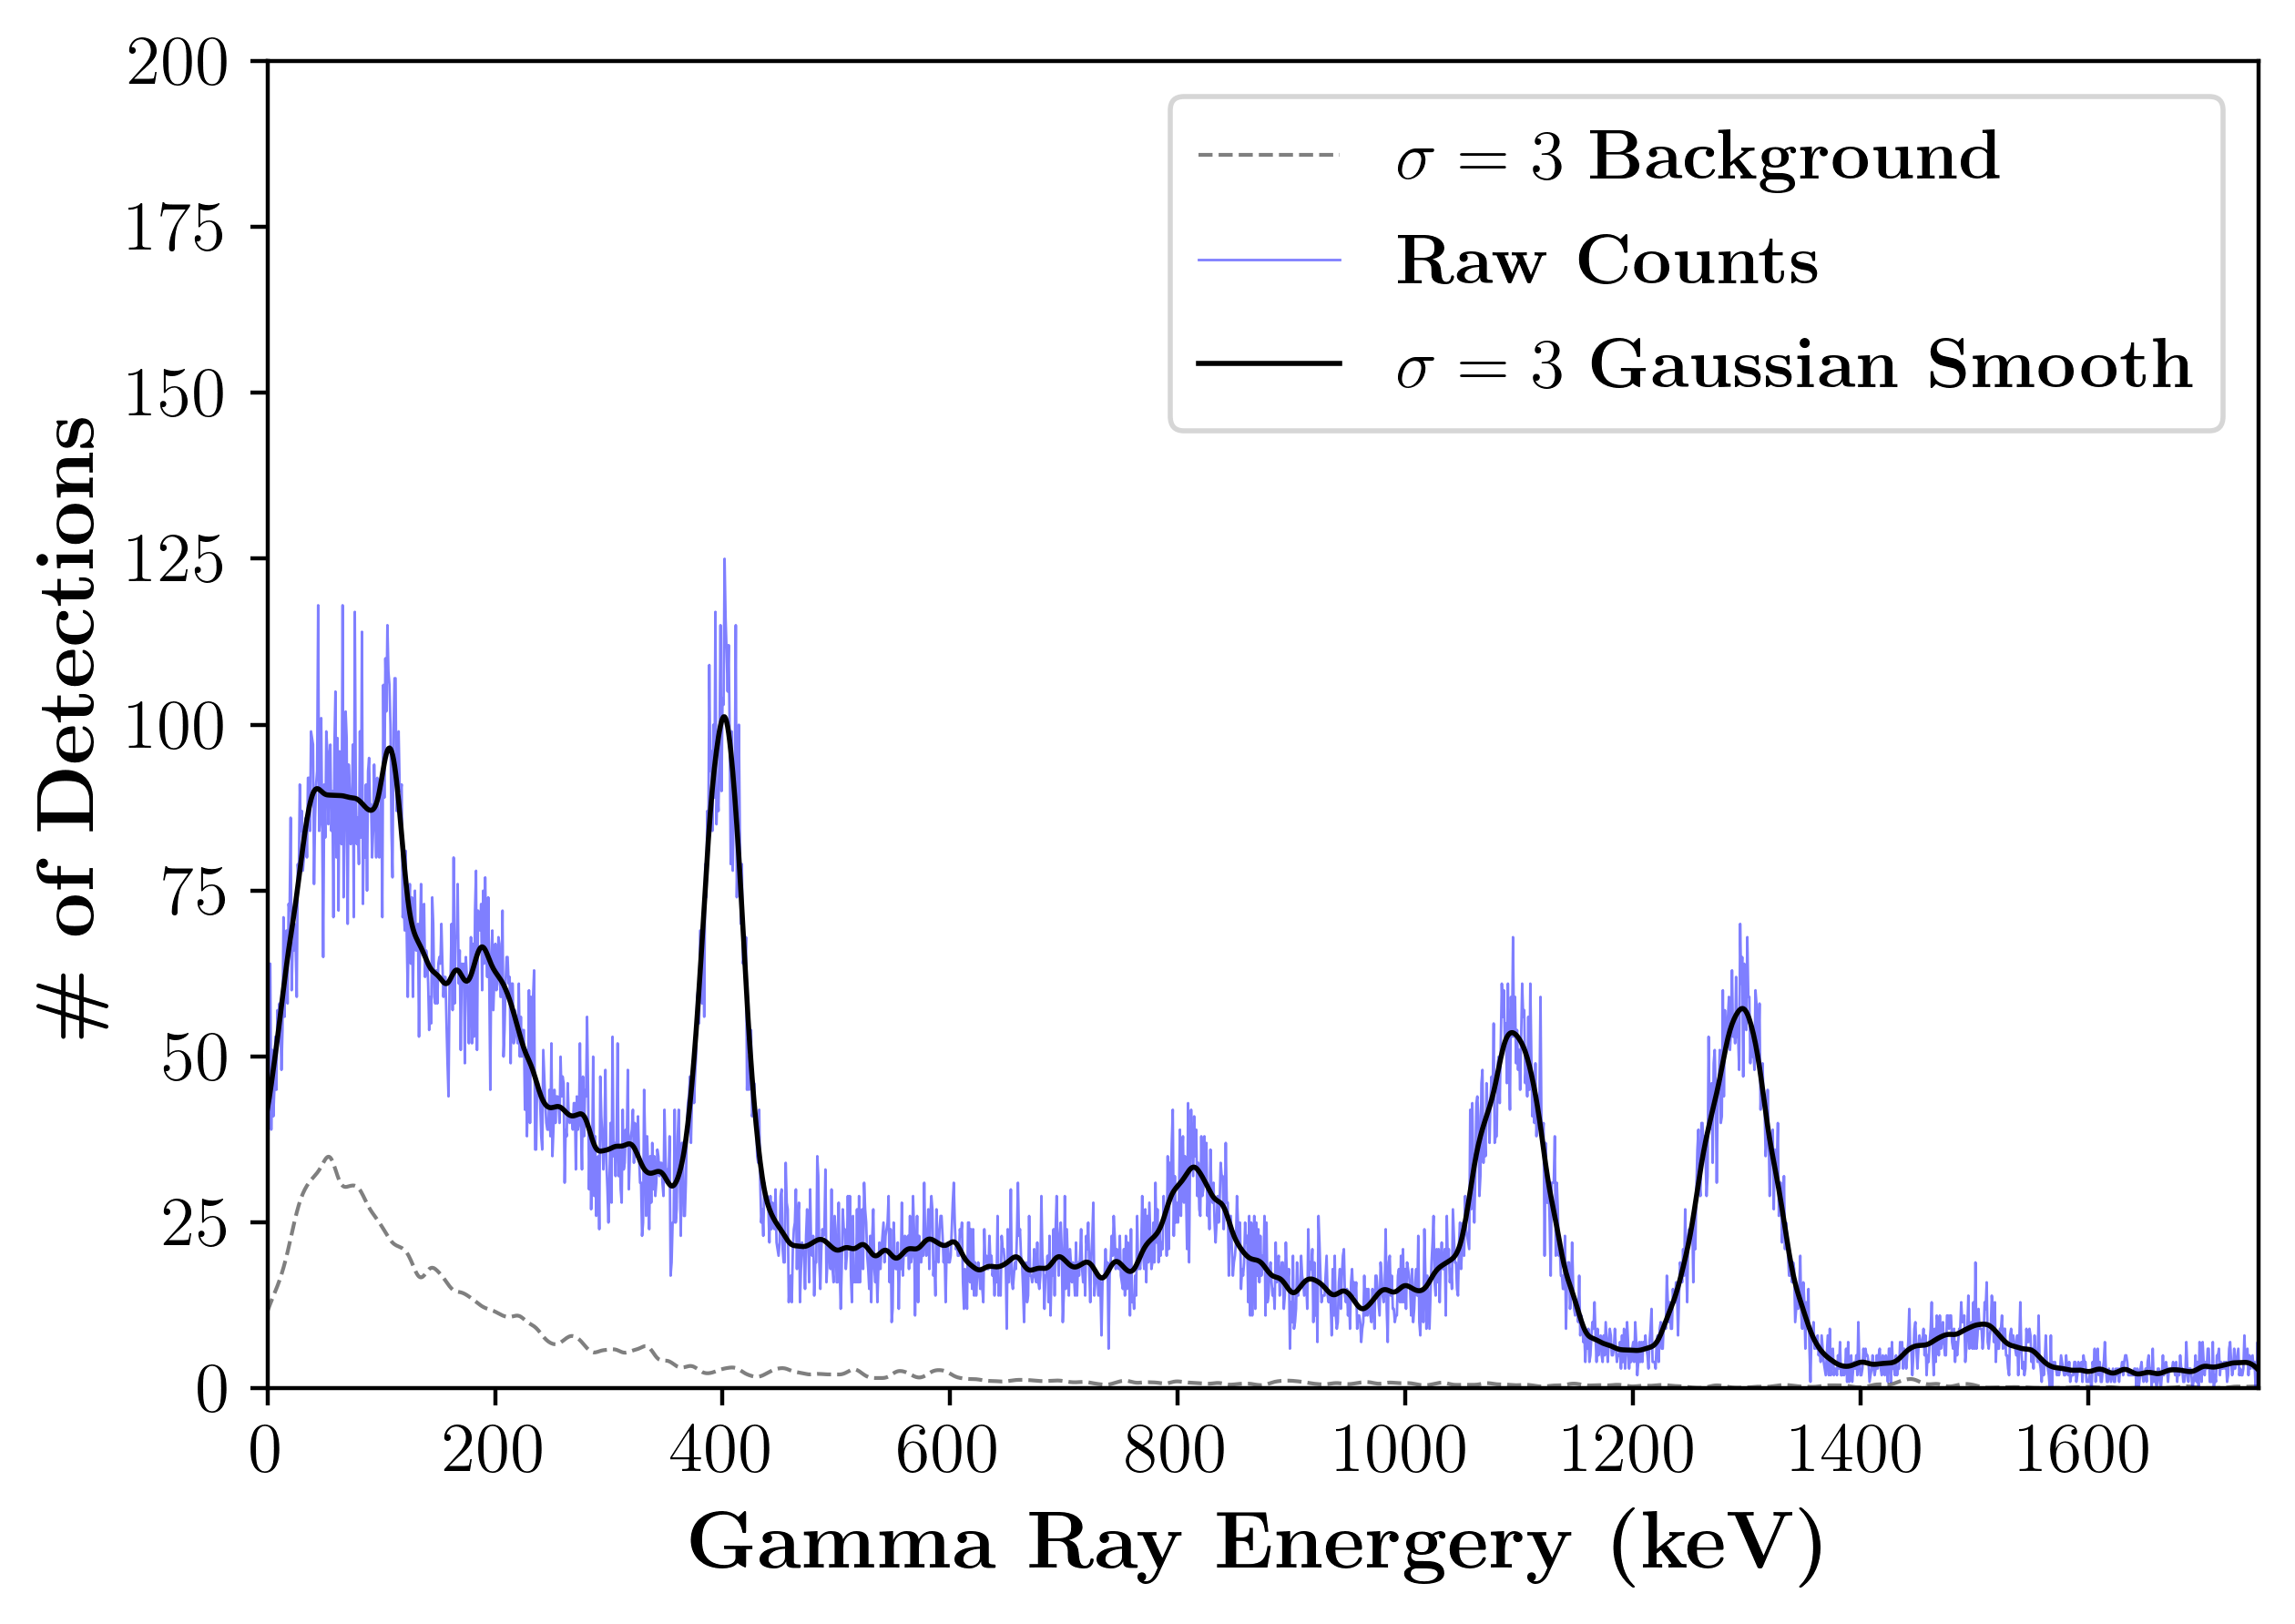
\includegraphics[width=0.49\textwidth]{figures/mystery_4_background_counts_overlay.png}}\\
        \subfloat[Recording 5, hh:mm:ss, $T+$ minutes\label{subfig:mystery-recording-5}]{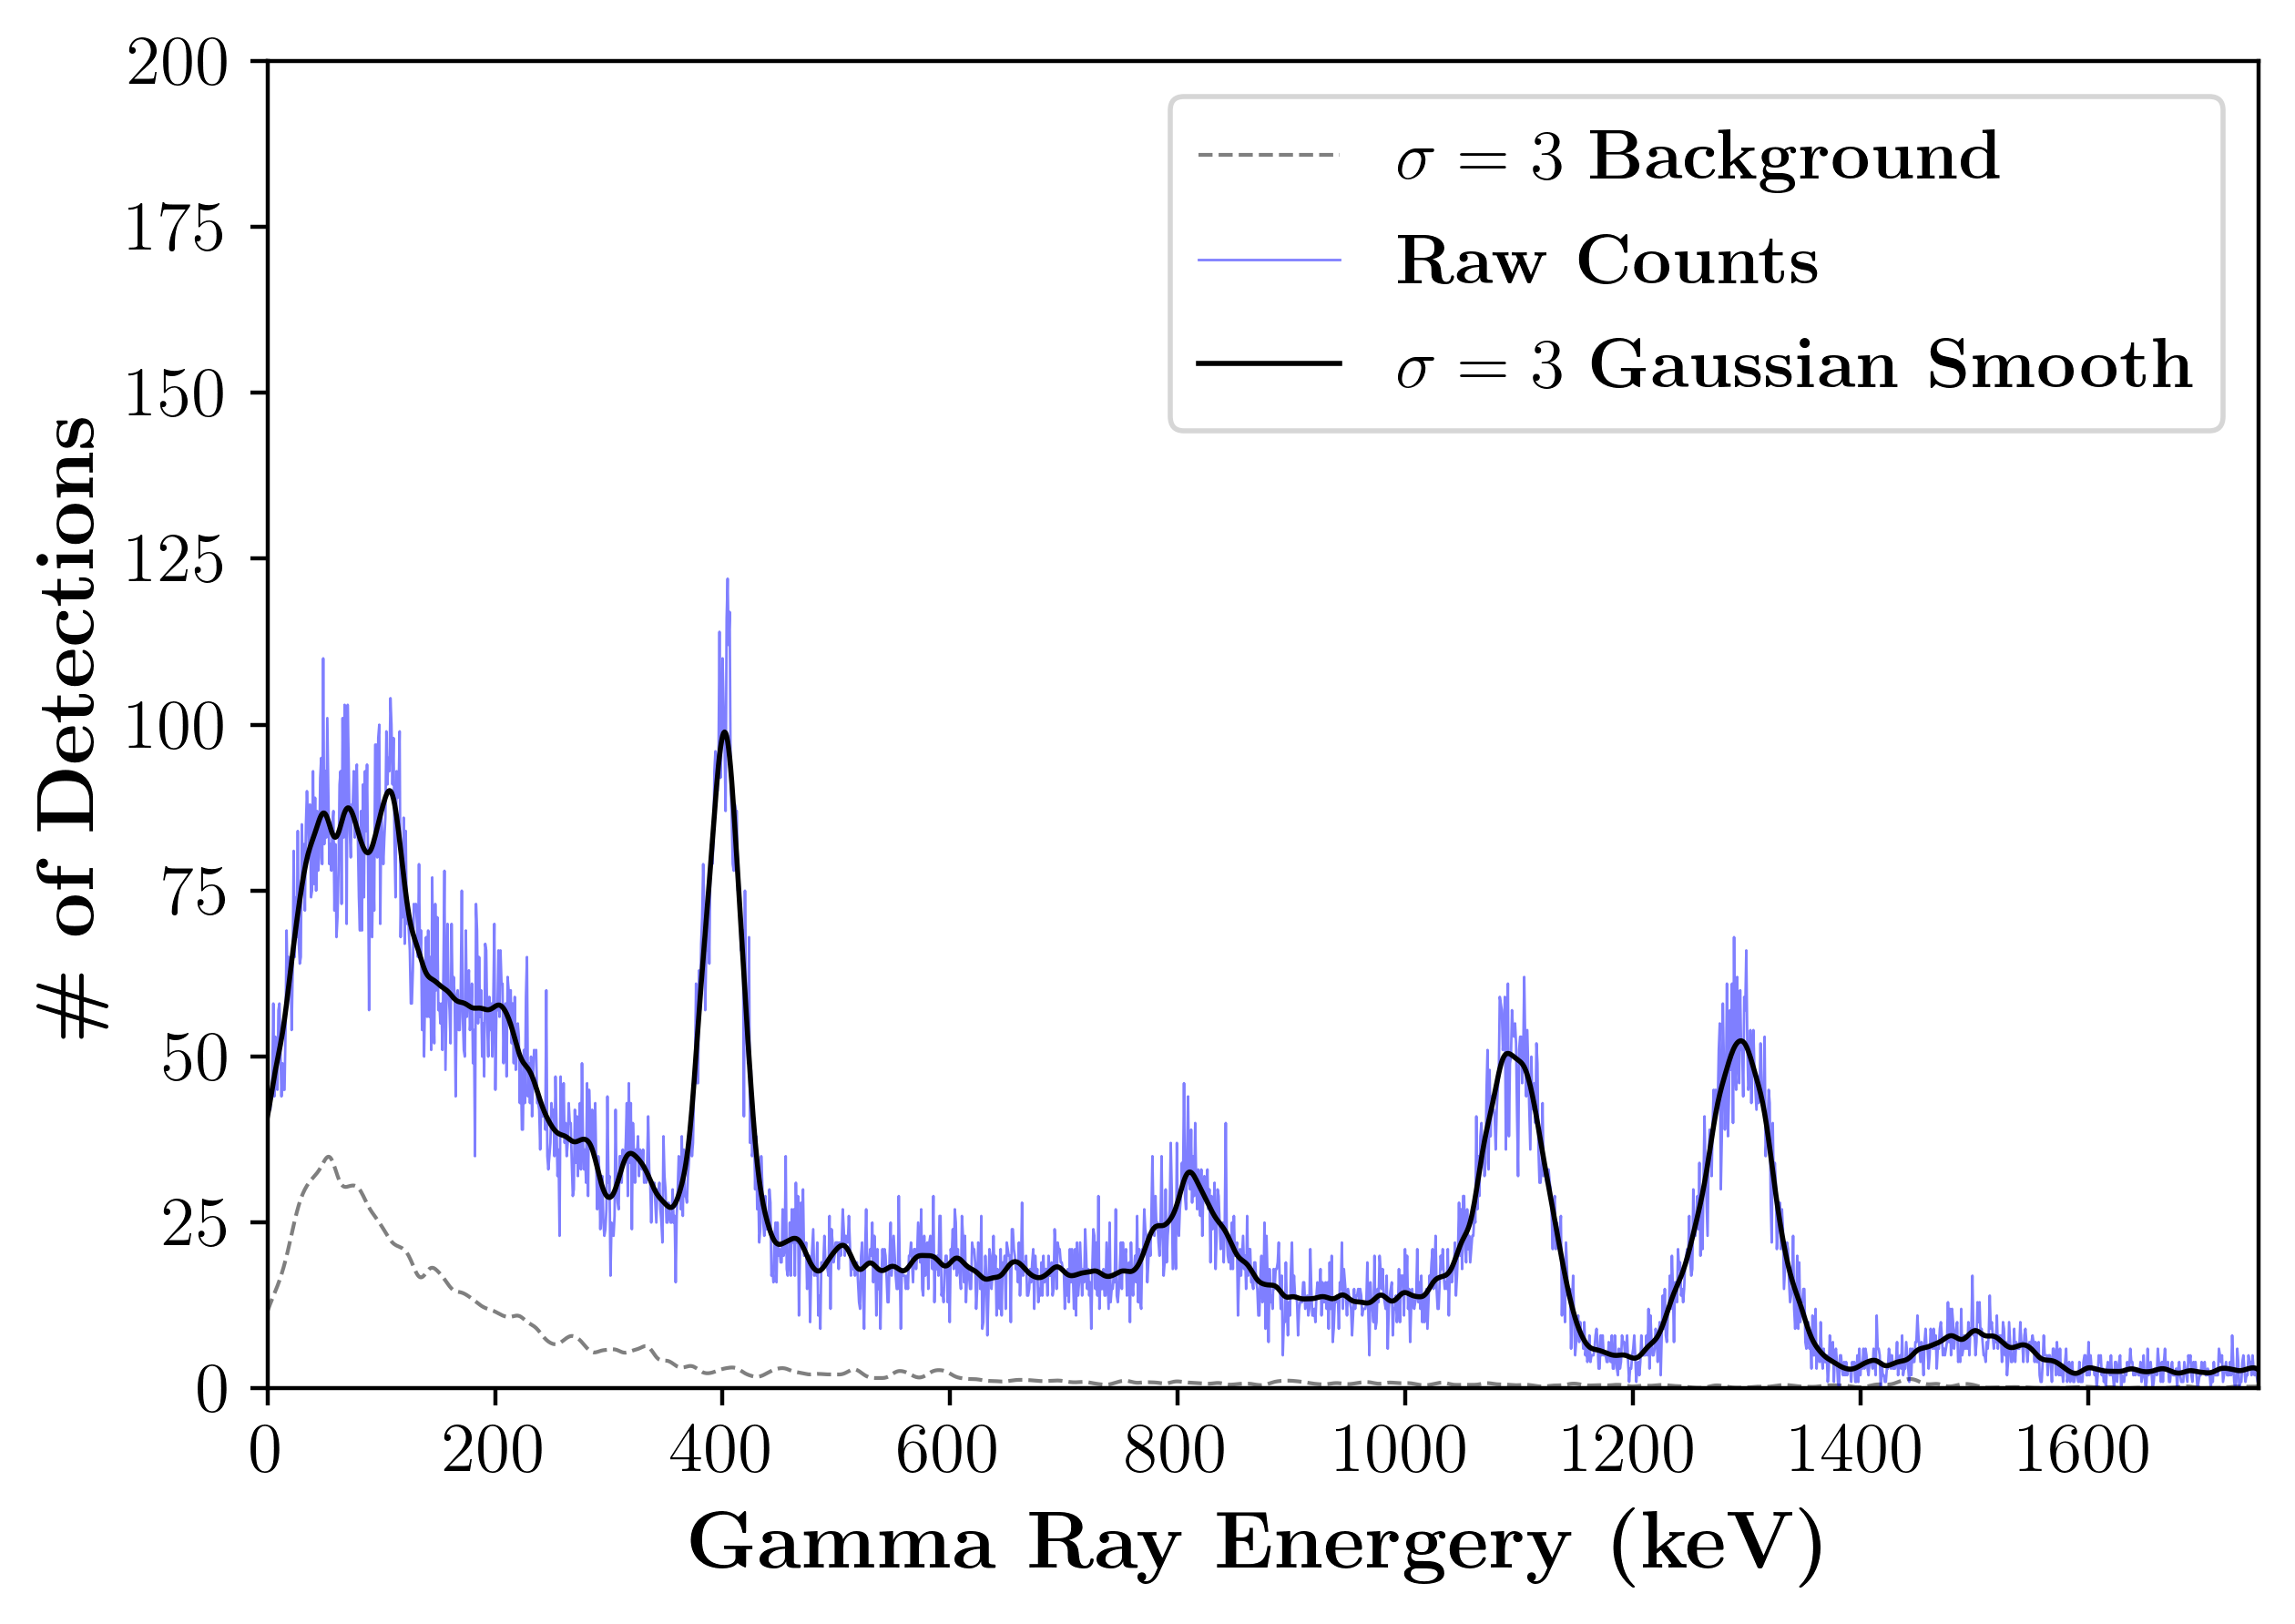
\includegraphics[width=0.49\textwidth]{figures/mystery_5_background_counts_overlay.png}}
        \hspace{\fill}
        \subfloat[Recording 6, hh:mm:ss, $T+$ minutes\label{subfig:mystery-recording-6}]{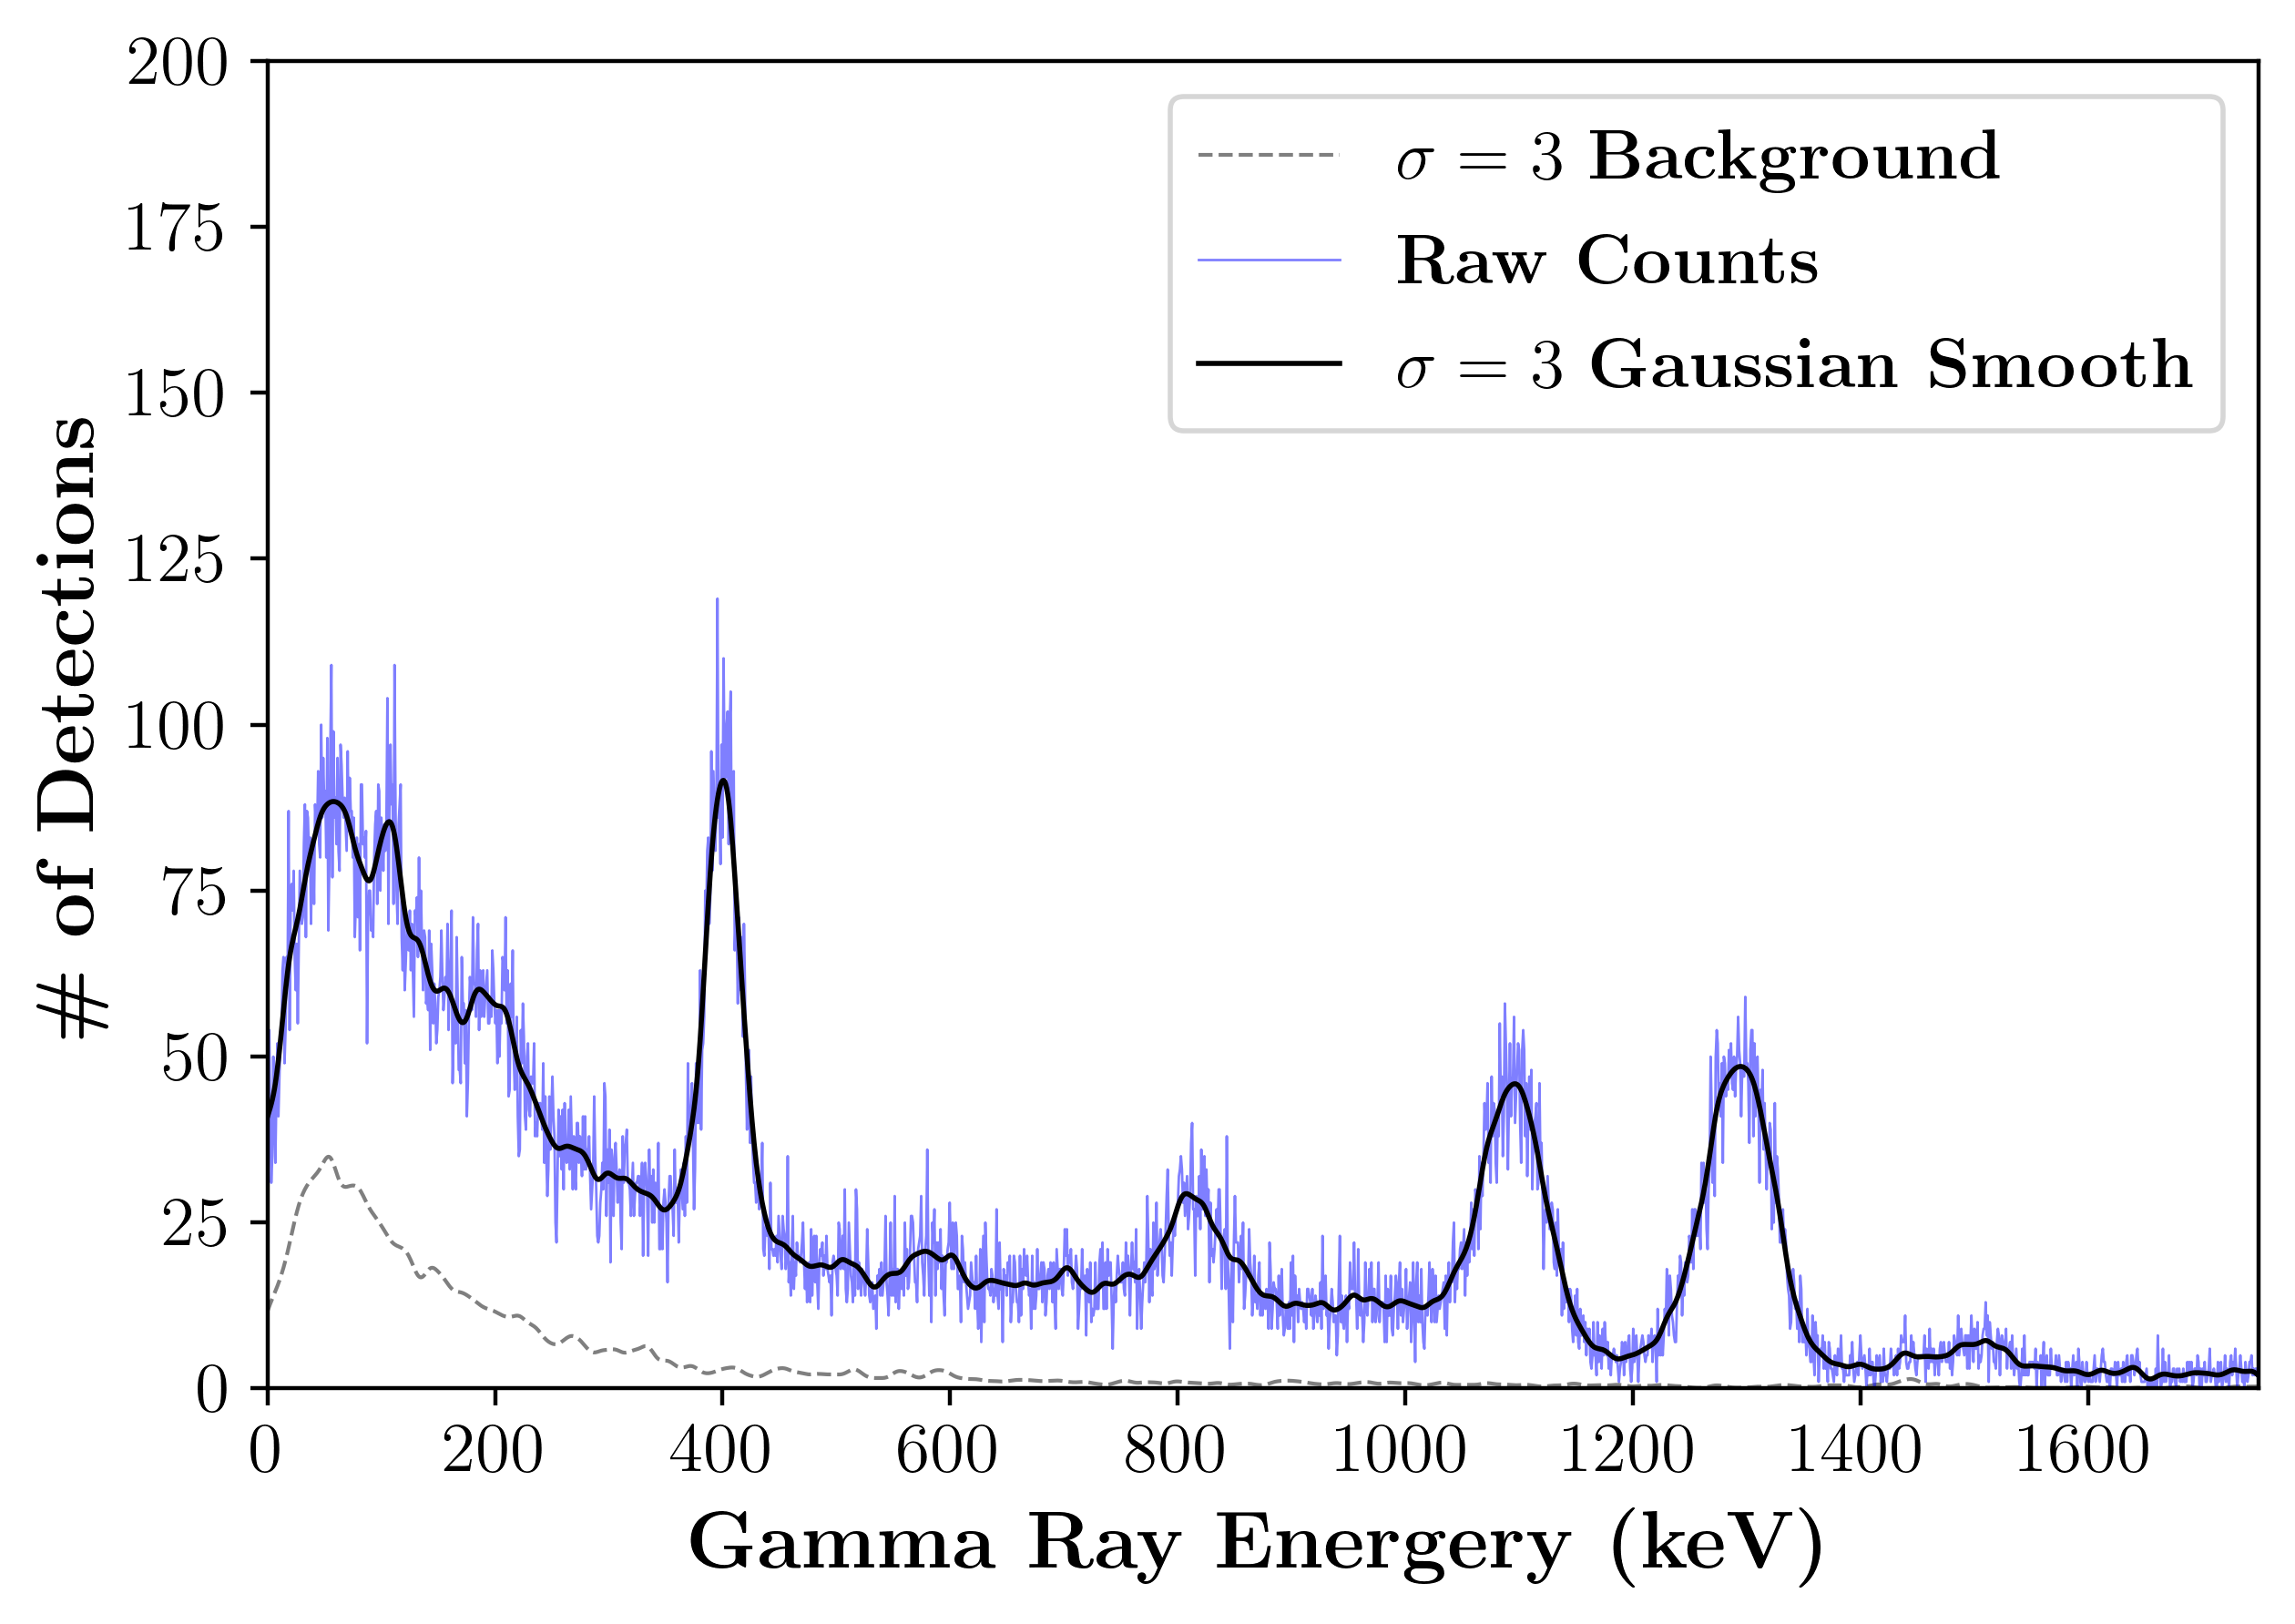
\includegraphics[width=0.49\textwidth]{figures/mystery_6_background_counts_overlay.png}}
        \caption{Raw count data for each recording of gamma rays from the unknown isotope.}
    \end{figure}
    ss
\end{document}